\chapter{Theory}
\label{chap:theory}
%\chapterquote{All science is either physics or stamp collecting.}
%{Ernest Rutherford}

This chapter explains the theoretical motivation for the Higgs boson, how it is produced at the \LHC and its decay into two photons. The convention $c=\hbar=1$ is assumed everywhere. Four vector indices are labelled by $\mu$ and $\nu$, whilst $i$, $j$, $k$ are used to label $SU(2)$ generators and $a$, $b$, $c$ used to label $SU(3)$ generators.

\section{The Standard Model}
\label{sec:standardmodel}

The \SM of Particle Physics is one of the crowning achievements of 20th century science. Its accuracy under high precision tests and prediction of subsequently observed phenomena in high energy physics is testament to its sucess. It is a gauge \QFT which provides a description of the fundamental particles of matter and three of the four known forces which govern their interactions; electromagnetism, the weak force and the strong force. Gravity is not included in the \SM but given the small scale nature of particle interactions and the relative weakness of gravity in comparison to the other forces its exclusion has a neglible impact on the predictive power of the \SM, at the energy scales of all experiments so far. 

\subsection{Fundamental particles and forces}

The fundamental matter particles described by the \SM, which compose all of the known matter in the universe, are spin-1/2 fermions which obey the Dirac equation,
\begin{equation}
  (i\gamma^{\mu}\partial_{\mu}\-m)\psi=0
  \label{eq:dirac}
\end{equation}
where $\gamma^{\mu}\gamma^{\nu}+\gamma^{\nu}\gamma^{\mu}=2\eta^{\mu\nu}$ and $\eta^{\mu\nu}$ is the Minkowski metric $(+,-,-,-)$~\cite{Halzen}.

The matter particles fall into two broad categories, those which interact with the strong force, the \textit{quarks}, and those which don't, the \textit{leptons}. When examining these particles in a table it is apparent there is some symmetry and beauty in their structure. There are six \textit{leptons}; the electron ($e$), muon ($\mu$), tau ($\tau$) and their corresponding neutrinos ($\nu_{e}$, $\nu_{\mu}$, $\nu_{\tau}$), and six \textit{quarks}; known as up, down, strange, charm, bottom and top ($u$, $d$, $s$, $c$, $b$, $t$). Each of them has a corresponding antiparticle equal in mass but with opposite charge. The \textit{quarks} are distinguished by their interaction with the strong-force which by its nature confines quarks to bound states. The strong force potential between two quarks contains a term linear in the distance between them, $r$. This overpowers the $1/r^{2}$ term, analagous to that in electromagnetism, such that the more energetically favourable solution for overcoming the potential is the creation of a new quark anti-quark pair. Consequently, quarks are never observed as free states but as composite particles (\textit{hadrons}) of two types; \textit{mesons}, which consist of a quark, anti-quark pair, and \textit{baryons}, which consist of quark triplets. The conserved currents of the strong force, analogous to the electromagnetic charge, are colour charge which are denoted red, green or blue. One realisation of quark confinement is that free observable states are colourless; mesons contain colour anti-colour pairs and baryons contain a quark of each colour. A summary of the matter fermions along with their masses and their electromagnetic charge is given in Table~\ref{tab:particles}.

\begin{table}[htb]
  \begin{tabular}{c | c l r | c l r }
  & \multicolumn{3}{c}{\textit{Leptons}} & \multicolumn{3}{c}{\textit{Hadrons}} \\
  Family & Particle      & Mass (MeV)  & Charge &  Particle      & Mass (MeV)  & Charge   \\
  \hline
  \multirow{2}{*}{I}    & $e^{-}$       & 0.511       & $-1$     &  $u$           & 2.3       & $+2/3$      \\
                        & $\nu_{e}$     & ~0          & 0      &  $d$           & 4.8         & $-1/3$       \\
  \multirow{2}{*}{II}   & $\mu^{-}$     & 105         & $-1$     &  $s$           & 95         & $+2/3$      \\
                        & $\nu_{\mu}$   & ~0          & 0      &  $c$           & 1.275~GeV          & $-1/3$       \\
  \multirow{2}{*}{III}  & $\tau^{-}$    & 1777        & $-1$     &  $b$           & 4.18~GeV        & $+2/3$      \\
                        & $\nu_{\tau}$  & ~0          & 0      &  $t$           & 173~GeV          & $-1/3$      \\
  \end{tabular}
  \caption[The fundamental matter particles]{The fundamental matter particles. Each particle is spin-1/2 and also has a corresponding anti-particle. All values taken from Ref.~\cite{pdg}.}
  \label{tab:particles}
\end{table}

The fundamental forces in the \SM act via the exchange of a spin-1 vector boson. For the electromagnetic force it is the photon, \gamma, for the weak force the $W^{\pm}$ and $Z$ bosons and for the strong the force the gluons, $G^{a}$, of which there are 8. The force-carrying particles are summarised in Table~\ref{tab:forces}. One noticeable difference is that the photon and gluons are massless whilst the $W^{\pm}$ and $Z$ have a large mass. This becomes something of a problem when trying to unify the electromagnetic and weak forces as we somehow need to generate mass terms for the heavy bosons without doing so for the photon whilst maintaining the symmetry in the system. In turns out this can be done using spontaneous symmetry breaking which gives rise to one other particle in the \SM which has not been mentioned yet, the Higgs boson. The next part of this chapter considers the symmetries involved in the \SM, how they can be broken, why it is necessary that they are and why this necessitates the existence of a massive scalar particle.

\begin{table}
  \begin{tabular}{c | c c c}
  Force & Particle & Mass (GeV) & Charge \\
  \hline
  Electromagnetic & $\gamma$ & 0 & 0 \\
  \multirow{2}{*}{Weak} & $W^{\pm}$ & 80.4 & $\pm$1 \\
                        & $Z$   & 91.2 & 0 \\
  Strong                & $G^{a}$   & 0 & 0 \\   
  \end{tabular}
  \caption[A summary of the fundamental force-carrying particles in the \acs{SM}]{A summary of the fundamental force-carrying particles in the \SM. All values taken from Ref.~\cite{pdg}.}
  \label{tab:forces}
\end{table}

\subsection{Gauge Theories}

Symmetry, and the mathematical dynamics of symmetry, are an incredibly important tool for describing fundamental physical principles. In 1918 Emmy N\"{o}ether proved that for each symmetry of the action of a physical system which can be written in the Lagrangian formalism there is a corresponding conserved quantity~\cite{noether,noether_trans}. Energy and momentum conservation are two typical examples of this which are particularly appropriate, and desirable, for particle physics. For any theory which is invariant under spatial translations (we should certainly demand that a physical principle follows the same laws anywhere in space) then N\"{o}ether's conserved quantity is momentum. For any theory which is invariant under time translations (we should also demand that a physical principle follow the same laws now, in the past and in a hundred years time) then the conserverd quantity is energy. Symmetry plays a particularly important role in the \SM because it is apparent that there are considerably more profound symmetries than those associated with space-time and furthermore that some of them can be broken. By demanding that any theory describing the particle structure of the universe has the appropriate conservation properties, the dynamics of theory can be constructed in the Lagrangian formalism by requiring that is invariant under the relevant symmetries. 

The \SM is a quantised gauge theory, which is to say that the \SM Lagrangian is invariant under certain local transformations. These are known as \textit{gauge symmetries} which form a symmetry group, also called a gauge group. For each independent degree of freedom in the symmetry group there exists a generator of the group which manifests itself in the theory as a vector field, also known as a gauge field, and for a quantum theory these are spin-1 bosons. These gauge fields must be included in the mathematical formalism of the Lagrangian to ensure its invariance under the local gauge transformations~\cite{Guidry}. This is manifested mathematically by substituting the derivative, $\partial^{\mu}$, in the Dirac equation (Eq.~\ref{eq:dirac}) for a covariant derivative,
\begin{equation}
  \partial_{\mu} \rightarrow D_{\mu} = \partial_{\mu}-igA_{\mu},
\end{equation}
where $A_{\mu}$ represents the gauge field required to maintain local invariance. In the \SM we recognise these gauge fields as the force-carrying particles described in Table~\ref{tab:forces}. This means that for each fundamental force present in the \SM there must be a corresponding symmetry which has the same number of independent group generators as there are gauge bosons. The \SM symmetry group is,
\begin{equation}
  SU(3) \otimes SU(2) \otimes U(1).
\end{equation}

The vector field required to maintain invariance under the $U(1)$ subgroup is labelled $B_{\mu}$, and the vector fields required to maintain invariance under the $SU(2)$ subgroup are labelled $W^{i}_{\mu}$, for $i=1,2,3$. Naively one might associate these to the \SM gauge bosons in Table~\ref{tab:forces}, however in reality nature is not as compartmentalised as this. For the proper physical description one needs to unify these two forces into the electroweak force, whose symmetry group is simply $SU(2)_{L}\otimes U(1)_{Y}$~\cite{Glashow,Weinberg,Salam}.  The physical states are written as,
\begin{align}
  & W_{\mu}^{\pm} = \frac{1}{\sqrt{2}}(W^{1}_{\mu}\mp iW^{2}_{\mu})\\
  & Z_{\mu} = \cos(\theta_{W})W^{3}_{\mu}-\sin(\theta_{W})B_{\mu}\\
  & A_{\mu} = \sin(\theta_{W})W^{3}_{\mu}+\cos(\theta_{W})B_{\mu}\\
\end{align}
where $A^{\mu}$ is the photon field and $\theta_{W}$ is known as the Weinberg angle which relates the coupling strengths of the weak, $g_{2}$, and electromagnetic, $g_{1}$, interactions,
\begin{equation}
  \frac{g_{1}}{g_{2}} = \frac{\sin(\theta_{W})}{\cos(\theta_{W})}.
\end{equation}
The generators for the $SU(2)$ part of the group are $T_{i}=\tau_{i}/2$, where $\tau_{i}$ for $i\in{1,2,3}$ are the Pauli spin matrices. There is one additional generator for the $U(1)$ part of the group, $Y$. The corresponding conserved quantities for these symmetries are weak isospin, $t_{1,2,3}$ and hypercharge, $y$ which are related to the electromagnetic charge, $Q$, by the relation, 
\begin{equation}
  Q = t_{3}+y/2,
\end{equation}
 and the factor of 2 is chosen by convention. The remaining $SU(3)$ sector requires 8 independent vector fields, the gluons $G_{\mu}^{a}$ for $a=1,2,3...8$, whose generators are given by the Gell-Mann matrices, $\lambda_{a}$ for $a\in{1,2,...,8}$, with the corresponding conserved quantity being colour charge. Thus the full covariant derivative is written as,
\begin{equation}
  D_{\mu} = \partial_{\mu}-ig_{1}\frac{Y}{2}B_{\mu} -ig_{2}\frac{\tau_{i}}{2}W_{\mu}^{i} -ig_{3}\frac{\lambda_{a}}{2}G_{\mu}^{a}.
  \label{eq:cov_der}
\end{equation}

\subsection{Quark and Lepton states}

The matter particles are spin-1/2 fermions and consequently labelled by spinor fields, $\psi$. These can be split into their left and right-handed chiral constituents using the projection operators, $P_{L}$ and $P_{R}$, such that $\psi_{L}=P_{L}\psi$ and $\psi_{R}=P_{R}\psi$.
The electroweak is a distinctly chiral force. Left and right-handed states transform differently under $SU(2)$ electroweak transformations. The former are electroweak singlets and the latter are electroweak doublets and for the first generation of leptons are written as,
\begin{align}
  \psi_{1} & = e_{R} &:SU(2)\;\;\;\;\mathrm{singlet} \\
  \psi_{2} & = L = \begin{pmatrix} \nu_{e} \\[-0.05cm] e \end{pmatrix}_{L} &:SU(2)\;\;\mathrm{doublet} 
\end{align}

Note that there is no right handed neutrino. The quarks are labelled in a similar way,
\begin{align}
  \psi_{3} & = u_{R\alpha} \\
  \psi_{4} & = d_{R\alpha} \\
  \psi_{5} & = Q_{L\alpha} = \begin{pmatrix} u_{\alpha} \\[-0.05cm] d_{\alpha} \end{pmatrix}_{L}  
\end{align}
where the additional index $\alpha$ describes the quark transformations in $SU(3)$ colour space. The convention is that whenever terms in the covariant derivative, Eq.~\ref{eq:cov_der}, act on fermion terms of a different matrix form they give zero. This allows the \SM fermion interaction Lagrangian to be written as,
\begin{equation}
  \mathcal{L} = \bar{\psi}i\gamma^{\mu}D_{\mu}\psi,
\end{equation}
where there is an implicit sum over the fermion types, $\psi_{i}$ for $i\in{1..5}=e_{R}, L, u_{R}, d_{R}, Q_{L}$, and a sum over the fermion generations. The kinetic term is simply written as,
\begin{equation}
  \mathcal{L} = -\frac{1}{4}F_{\mu\nu}F^{\mu\nu} = -\frac{1}{4}\biggl( B_{\mu\nu}B^{\mu\nu} + \mathrm{Tr} (W_{\mu\nu}W^{\mu\nu}) + \mathrm{Tr} (G_{\mu\nu}G^{\mu\nu}) \biggr),
\end{equation}
where $B_{\mu\nu}$, $W_{\mu\nu}^{i}$ and $G_{\mu\nu}^{a}$ are the field strength tensors for the three \SM gauge groups, which can be expressed in terms of their corresponding vector fields by the relation, 
\begin{equation}
X^{a}_{\mu\nu} = \partial_{\mu}A^{a}_{\nu}-\partial_{\nu}A^{a}_{\mu}+gf^{abc}A^{b}_{\mu}A^{c}_{\nu},
\end{equation}
where $f^{abc}$ is the structure constant of the particular group in question (one of $U(1)$, $SU(2)$ or $SU(3)$) and describes the commutation relationship between the group generators. %This is what makes the \SM a Yang-Mills gauge theory~\cite{YangMills}.

\subsection{Electroweak symmetry breaking}

As presented so far the \SM Lagrangian has no mass terms included in it but this is clearly in contention with our observation that most of the fundamental fermions and bosons have masses. Including mass terms by hand, of the form $m\bar{\psi}\psi$ for the fermions and $\frac{1}{2}m^{2}B^{\mu}B_{\mu}$ for the bosons, would explicitly break the $SU(2)$ invariance and consequently is not a good solution. The reason for this is that the electroweak is specifically a left handed force; there is no electroweak coupling to right handed fermions. An $SU(2)$ doublet, $\phi$, is required so that one can include a mass term which looks like $m\bar{L}\phi e_{R}$ and preserves invariance under $SU(2)$. There is a way to include a field exactly like this by spontaneously breaking the symmetry such that the Lagrangian itself is still invariant whilst its vacuum state, and hence particle spectrum, is not. It turns out that this mechanism generates a mass for the massive gauge bosons whilst leaving the photon massless and predicts the existence of a massive scalar particle. One can then introduce a coupling term for this new particle with the matter fermions which dictates the size of their masses. This is known as the Higgs mechanism.

An additional term is required in the \SM Lagrangian which introduces the Higgs field, an $SU(2)$ doublet, $\phi$,
\begin{equation}
  \mathcal{L} = T - V = (D^{\mu}\phi)^{\dagger}(D_{\mu}\phi) + \mu^{2}\phi^{\dagger}\phi - \lambda(\phi^{\dagger}\phi)^{2},
  \label{eq:higgs_potential}
\end{equation}
where $T$ and $V$ are the kinetic and potential terms respectively. We can study the particle spectrum by first finding the minimum of the potential, i.e. the vacuum state, and then expanding around this. By requiring that $\mu^{2}<0$ and $\lambda>0$ it is apparent that the potential is a Mexican hat shape whose minimum is non-zero and maps out a circle in the $SU(2)$ phase space. The vacuum state can be chosen as any one of these equivalent solutions, which lie along the circle, but the convention is to pick a direction, which anyway doesn't matter as the potential only contains terms in $\phi^{\dagger}\phi$, and define the \VEV as,
\begin{equation}
  \bra{0}\phi\ket{0} = \begin{pmatrix} 0 \\ \sqrt{-\dfrac{\mu^{2}}{2\lambda}} \end{pmatrix} = \frac{1}{\sqrt{2}} \begin{pmatrix} 0 \\ v \end{pmatrix}.
\end{equation}
The \VEV now breaks the $SU(2)$ invariance although the extra Lagrangian term introduced in Eq.~\ref{eq:higgs_potential} does not. The convention then considers small pertubations around the \VEV,
\begin{equation}
  \phi = \dfrac{1}{\sqrt{2}}\begin{pmatrix} 0 \\ v+H \end{pmatrix}.
\end{equation}
Inserting this definition of the field \phi into the Lagrangian given in Eq.~\ref{eq:higgs_potential}, where the covariant derivative, $D^{\mu}$, is defined in Eq.~\ref{eq:cov_der} (recall that the notation used was such that the $SU(3)$ operators $\lambda^{a}G^{a}_{\mu}$ operating on an $SU(2)$ state, such as \phi, gave zero) gives,
\begin{align}
  \mathcal{L} = & \frac{1}{2}(\partial^{\mu}H)(\partial_{\mu}H) - \mu^{2}H^{2} + \frac{1}{8}g_{2}^{2}v^{2}\Bigl(|W_{\mu}^{+}|^{2}+|W_{\mu}^{-}|^{2}\Bigr) +\frac{1}{8}g_{2}^{2}v^{2}\biggl[1+\Bigl(\frac{g_{1}}{g_{2}}\Bigr)^{2}\biggr]|Z^{0}_{\mu}|^{2} \nonumber\\ 
  & + \mbox{interaction terms} 
\end{align}
Only the relevant kinematic and mass terms here have been kept and all others are simply referred to as ``interaction terms". The spontaneous symmetry breaking mechanism has given rise to:

\begin{itemize}
  \item A scalar field, $H$, with mass, $m_{H} = \sqrt{-2\mu^{2}}$
  \item Two charged gauge boson fields, $W^{\pm}$, with the same mass, $m_{W} = g_{2}v/2$
  \item A neutral gauge boson field, $Z$, with mass, $m_{Z} = m_{W}\sqrt{1+\Bigl(g_{1}/g_{2}\Bigr)^{2}}$
  \item Notice that the neutral gauge boson field, $A_{\mu}$, has no mass term
\end{itemize}

Consequently a mass term has been generated for the $W^{\pm}$ and $Z$ bosons whilst the photon has been left massless. There is also the prediction of the \SM Higgs boson. By adding $SU(2)$ invariant Yukawa coupling terms in the Lagrangian, the fermion masses can also be generated by the Higgs boson. These terms are of the form,
\begin{equation}
  \mathcal{L} = k_{e} \Bigl( \bar{L}\phi e_{R} + \phi^{\dagger}\bar{e}_{R} L \Bigr) + \Biggl[ k_{d}\bar{Q}_{L}\phi d_{R} + k_{u}\bar{Q}_{L}(-i\tau_{2}\phi^{\star})u_{R} + \mathrm{h.c.} \Bigg],
\end{equation}
where h.c.~represents the hermitian conjugate of the preceeding terms in brackets and $k_{e,u,d}$ are the Higgs-fermion couplings which are directly related to the mass of the fermions by $m_{f}=k_{f}v/\sqrt{2}$. Neither the value of these couplings nor even the presence of such terms is determined by the gauge principle but they allow the theory to accomodate non-zero fermion masses via the Higgs boson. The relationship between the experimentally observed fermion masses and these couplings allow indirect constraints and properties of the Higgs boson to be calculated. The full \SM Lagrangian can be written by summing all the terms previously discussed and simplified to,
\begin{equation}
  \mathcal{L} = -\frac{1}{4}F_{\mu\nu}F^{\mu\nu} + \bar{\psi}i\gamma^{\mu}D_{\mu}\psi + |D\phi|^{2} +\mu^{2}|\phi|^{2} -\lambda|\phi|^{2} + [ \psi_{i}k_{ij}\psi_{j}\phi + \mathrm{h.c} ].
\end{equation}


This last section summarises the work of many: Higgs, Englert, Brout, Guralnik, Hagen, Kibble, Anderson, Nambu and Goldstone on spontaneous symmetry breaking and mass emergence~\cite{englert-brout,HagenKibble,Higgs:1964ia,Higgs,Nambu,Goldstone,Anderson}, Glashow, Weinberg and Salam on the electroweak model~\cite{Glashow,Weinberg,Salam} and t'Hooft and Veltman on the renormalisability and unitarity of the \SM~\cite{tHooft:1972fi,Hooft1971167}. It is quite amazing that using this model of electroweak symmetry breaking allowed Glashow, Weinberg and Salam to predict the existence, and the masses, of the $W^{\pm}$ and $Z$ bosons. These were experimentally observed by UA1 and UA2 experiments in 1983~\cite{ua1,ua2}. The theory also predicts the existence of a massive scalar boson known as the Higgs. Whilst its mass could not be directly predicted by the theory, various precision measurements made in the run up to \LHC operation suggested its mass would be light enough to be found, if the \SM was to be believed, at the energy scale of the \LHC. The rest of this chapter concentrates on Higgs production at the \LHC and its decay to two photons. 

\section{Higgs production at the \LHC}

The \LHC is predominantly a proton-proton collision machine capable of centre-of-mass energies far greater than any previous experiments. The dataset used for this thesis is taken at centre-of-mass energies, $\sqrt{s}=7$ and 8~\TeV. One of the experimental aims of the \LHC was to find the Higgs boson or provide clues about why it cannot be seen or does not exist. Theoretical constraints, before \LHC data taking, set an upper bound on the \SM Higgs mass of $\mH\leq710\pm60$~\GeV~\cite{upper-higgs-bound}. Previous searches by the \LEP experiment suggest a lower bound of $\mH\geq114.4$~\GeV at the 95\% confidence level~\cite{lep-higgs}. The \LHC should be very capable of producing \SM Higgs bosons anywhere in this mass range. The global electroweak precision fit for the Higgs mass prior to \LHC data suggested a \SM Higgs boson in the $1\sigma$ interval $[69-183]$~\GeV~\cite{ewfits}.

At the \LHC \SM Higgs bosons are produced predominantly in one of four ways: \ggH, \VBF\footnote{sometimes also referred to as qqH}, \VH\footnote{sometimes also split into \WH and \ZH separately} and \ttH. The Feynman diagrams for these processes are shown at leading order in Fig.~\ref{fig:feyn_prod}. As the Higgs only couples to mass, the gluon fusion production is apparent through a top loop. This is the most dominant production process, nearly 90\% of Higgs bosons produced at the \LHC come from gluon fusion, and provides a good measure of the Higgs coupling to fermions. The other three production modes are much smaller in cross section. However in these cases the production is in association with other particles which can be ``tagged" to provide additional sensitivity to an analysis by reducing the background rate. The \VBF production mode has a very specific topology. The associated quarks emitted in the production typically produce two high momentum but very forward jets which have a large spatial separation (in other words are back-to-back). The Higgs produced by this mechanism also typically has a large transverse momentum. The \VH production modes are associated with a $W^{\pm}$ or $Z$ boson so can be probed by searching for Higgs decays which also contain leptons and neutrinos, the latter measured at the \LHC as missing transverse energy (\MET). The \ttH production mode is associated to a pair of top quarks so can be probed by searching for Higgs decays containing $b$ quarks, leptons and \MET, as the decay chain used for a top quark is $t\rightarrow bW(\rightarrow l\nu)$.

\begin{figure}
  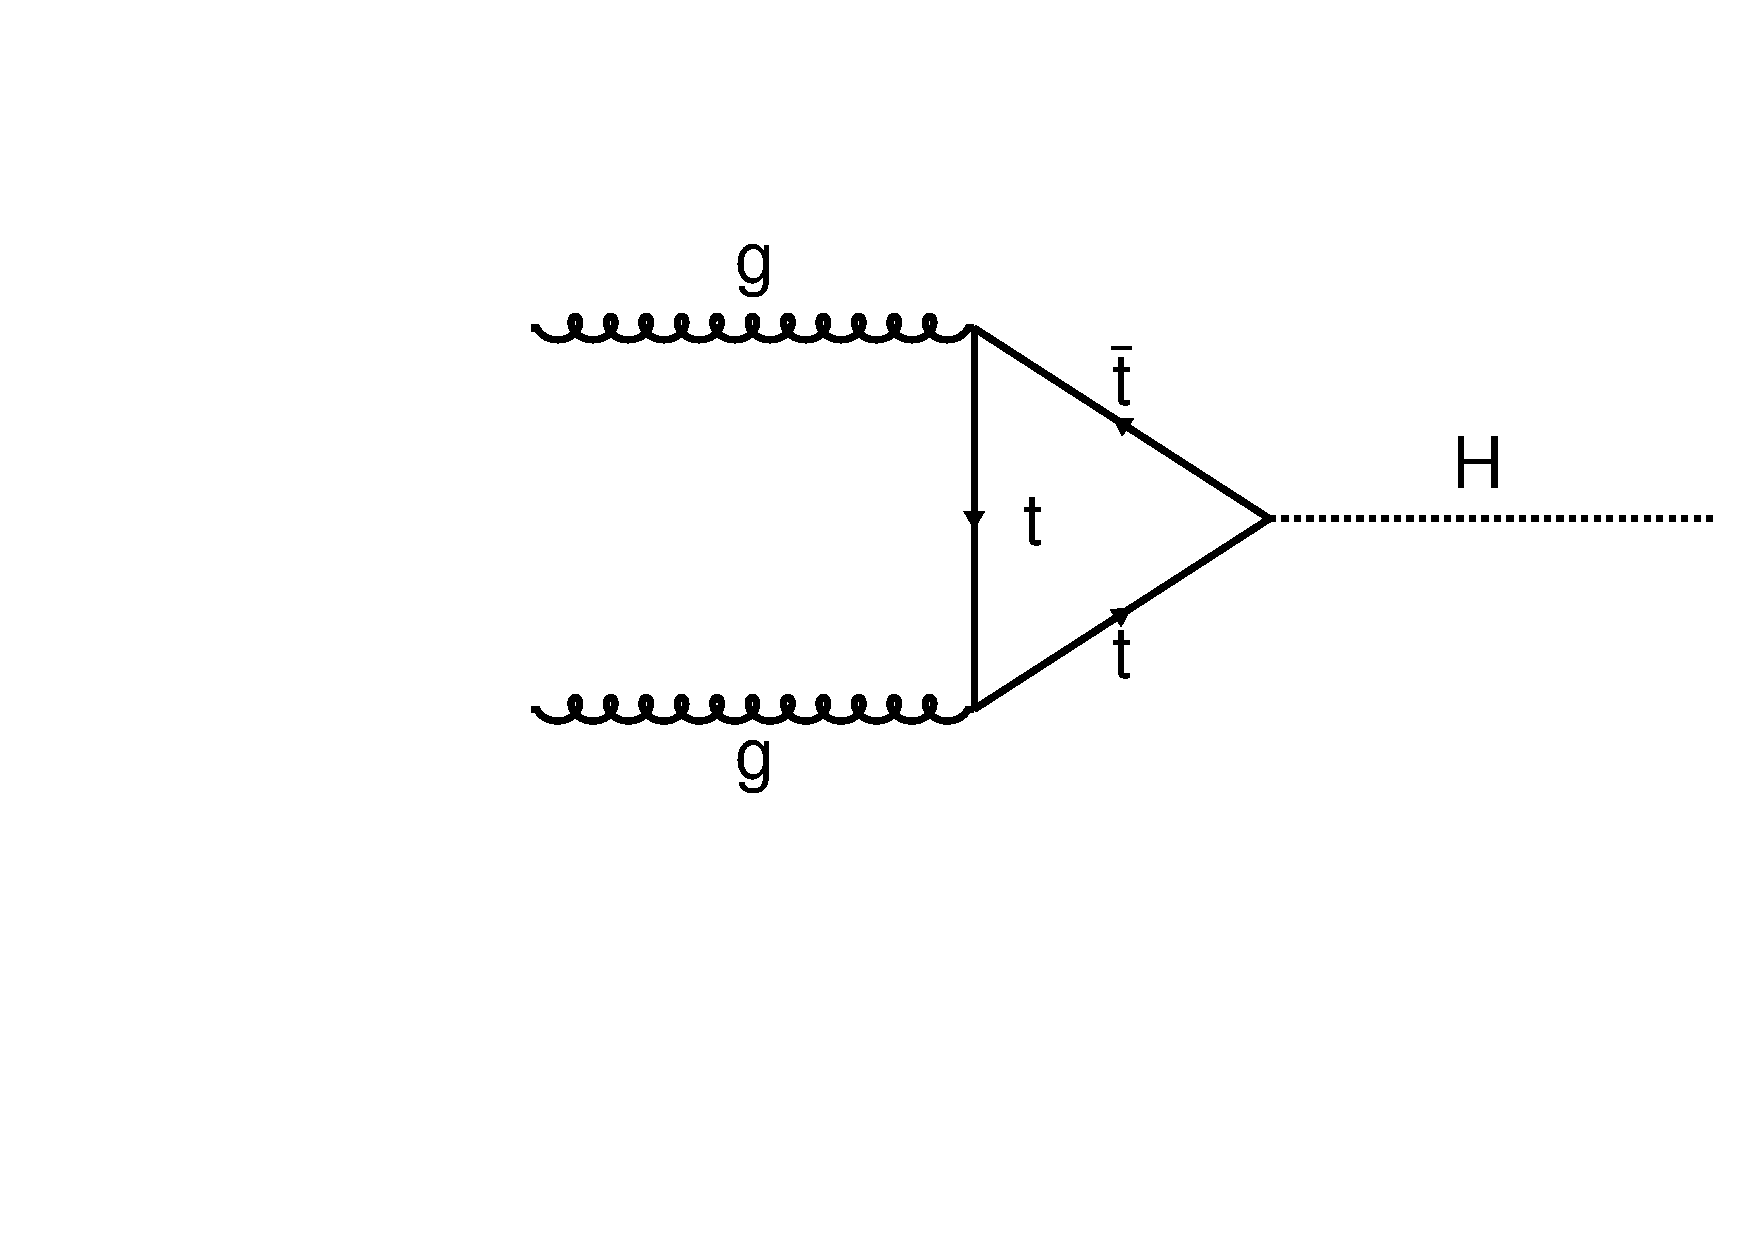
\includegraphics[width=0.45\textwidth]{theory/plots/ggh.pdf}
  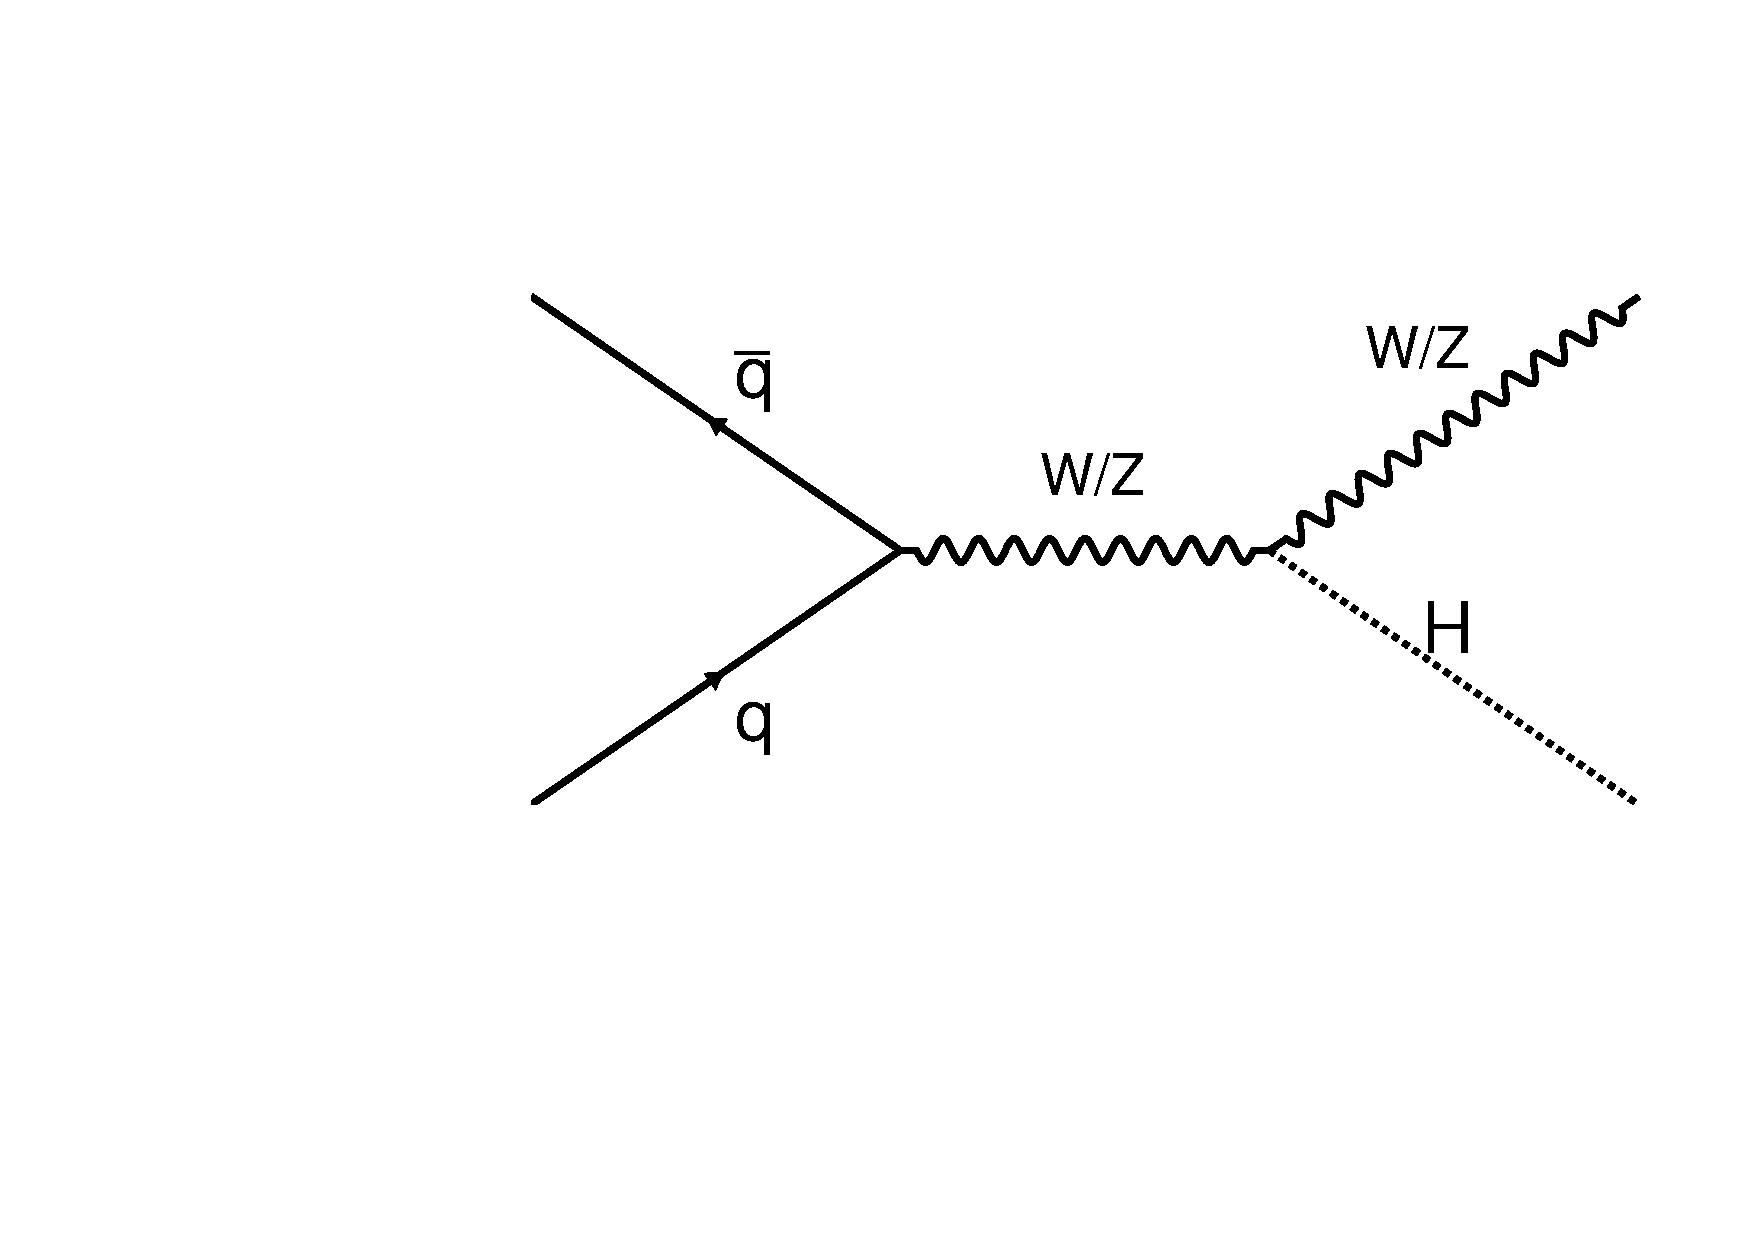
\includegraphics[width=0.45\textwidth]{theory/plots/vh.pdf}\\
  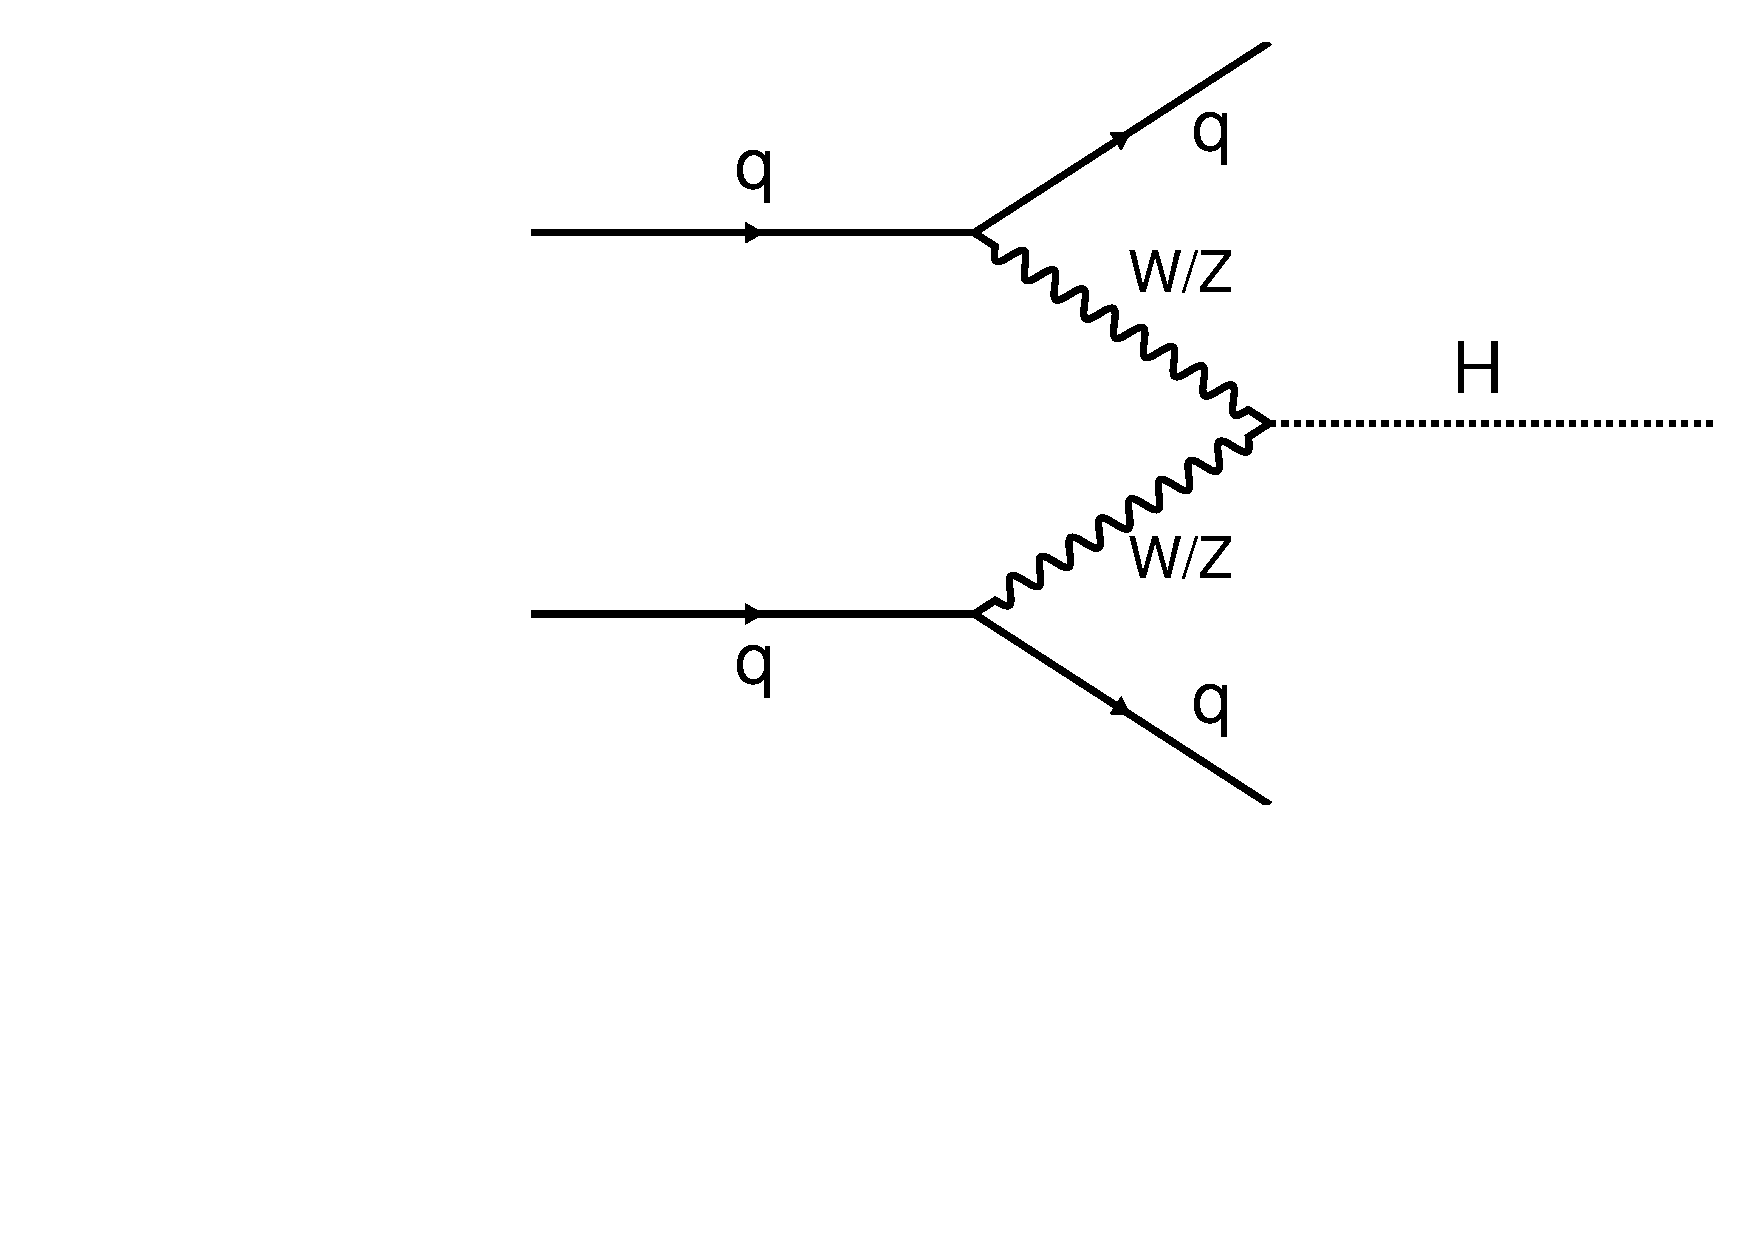
\includegraphics[width=0.45\textwidth]{theory/plots/qqh.pdf}
  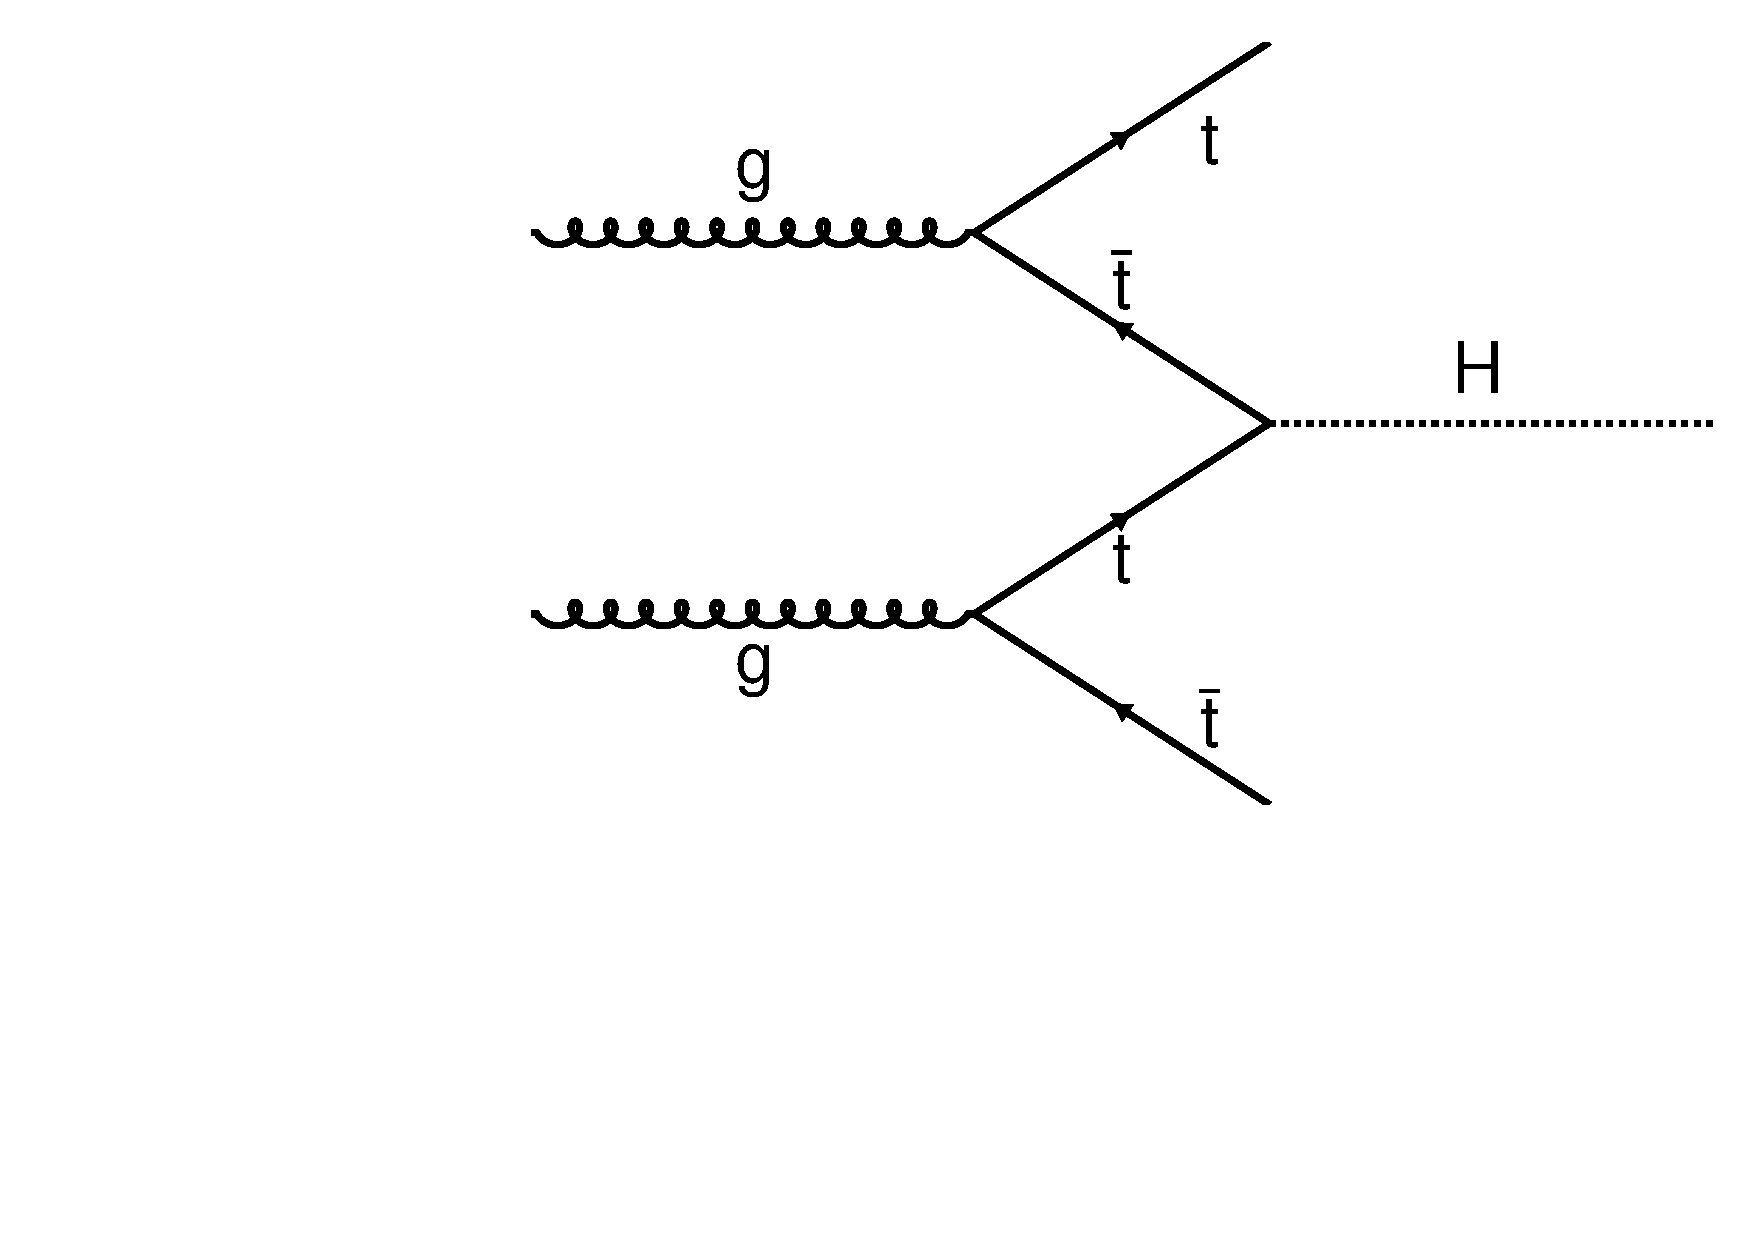
\includegraphics[width=0.45\textwidth]{theory/plots/tth.pdf}
  \caption[Feynman diagrams for \acs{SM} Higgs production at the \acs{LHC}]{The four main \SM Higgs production mechanisms at the LHC: gluon fusion (top left), vector boson fusion (bottom left), $W^{\pm}$ and $Z$ boson associated production (top right) and top anti-top annihilation (bottom right). The cross sections for each of these processes in proton-proton collisions is show in Fig.~\ref{fig:higgs_xs}.}
  \label{fig:feyn_prod}
\end{figure}

A demonstration of the differences between \ggH and \VBF production is shown in Fig.~\ref{fig:gen_level}. The generator level distributions of these two signals are shown as a function of the generated Higgs transverse momentum and generated Higgs pseudorapidity, \eta, defined as $\eta=-\ln\tan(\theta/2)$, where $\theta$ is the polar angle measured from the beam axis. 
\begin{figure}
  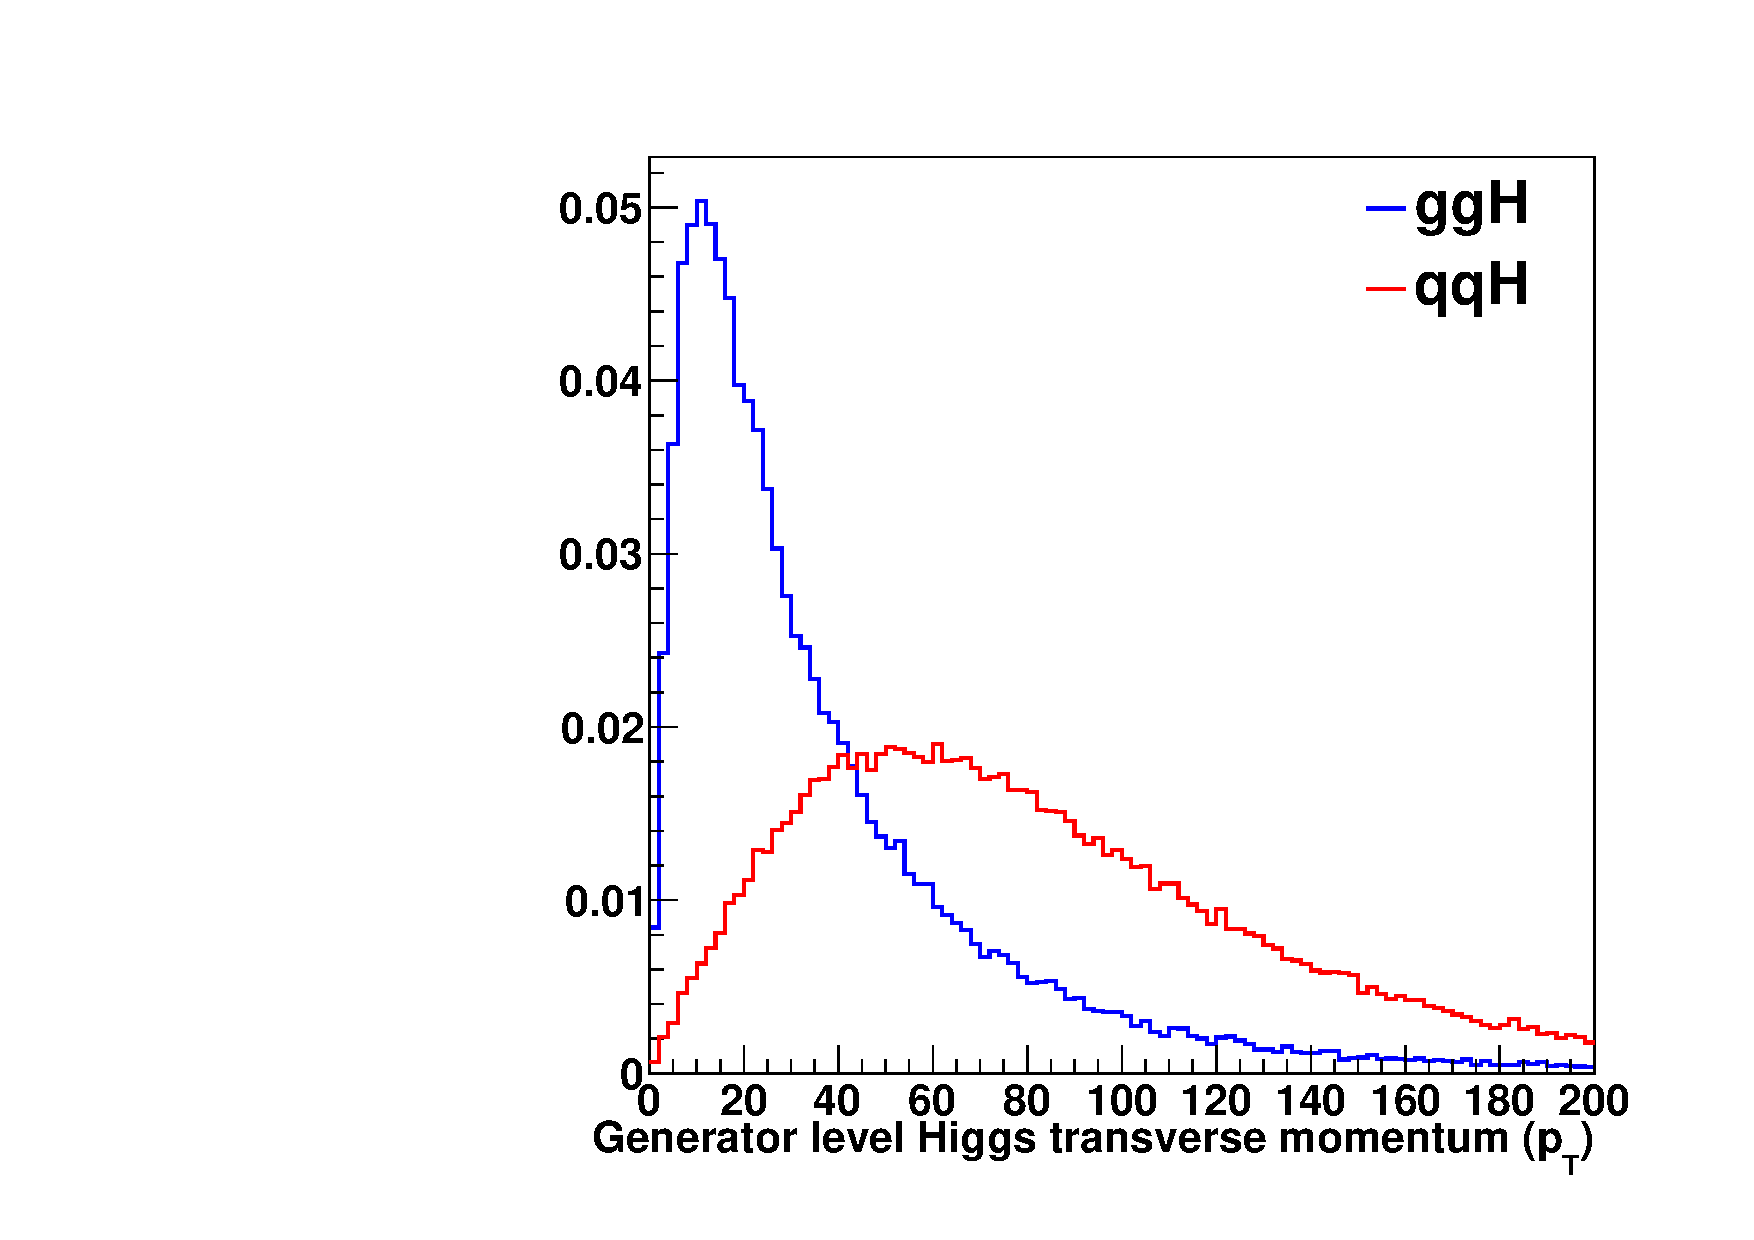
\includegraphics[width=0.45\textwidth]{theory/plots/genPT.pdf}
  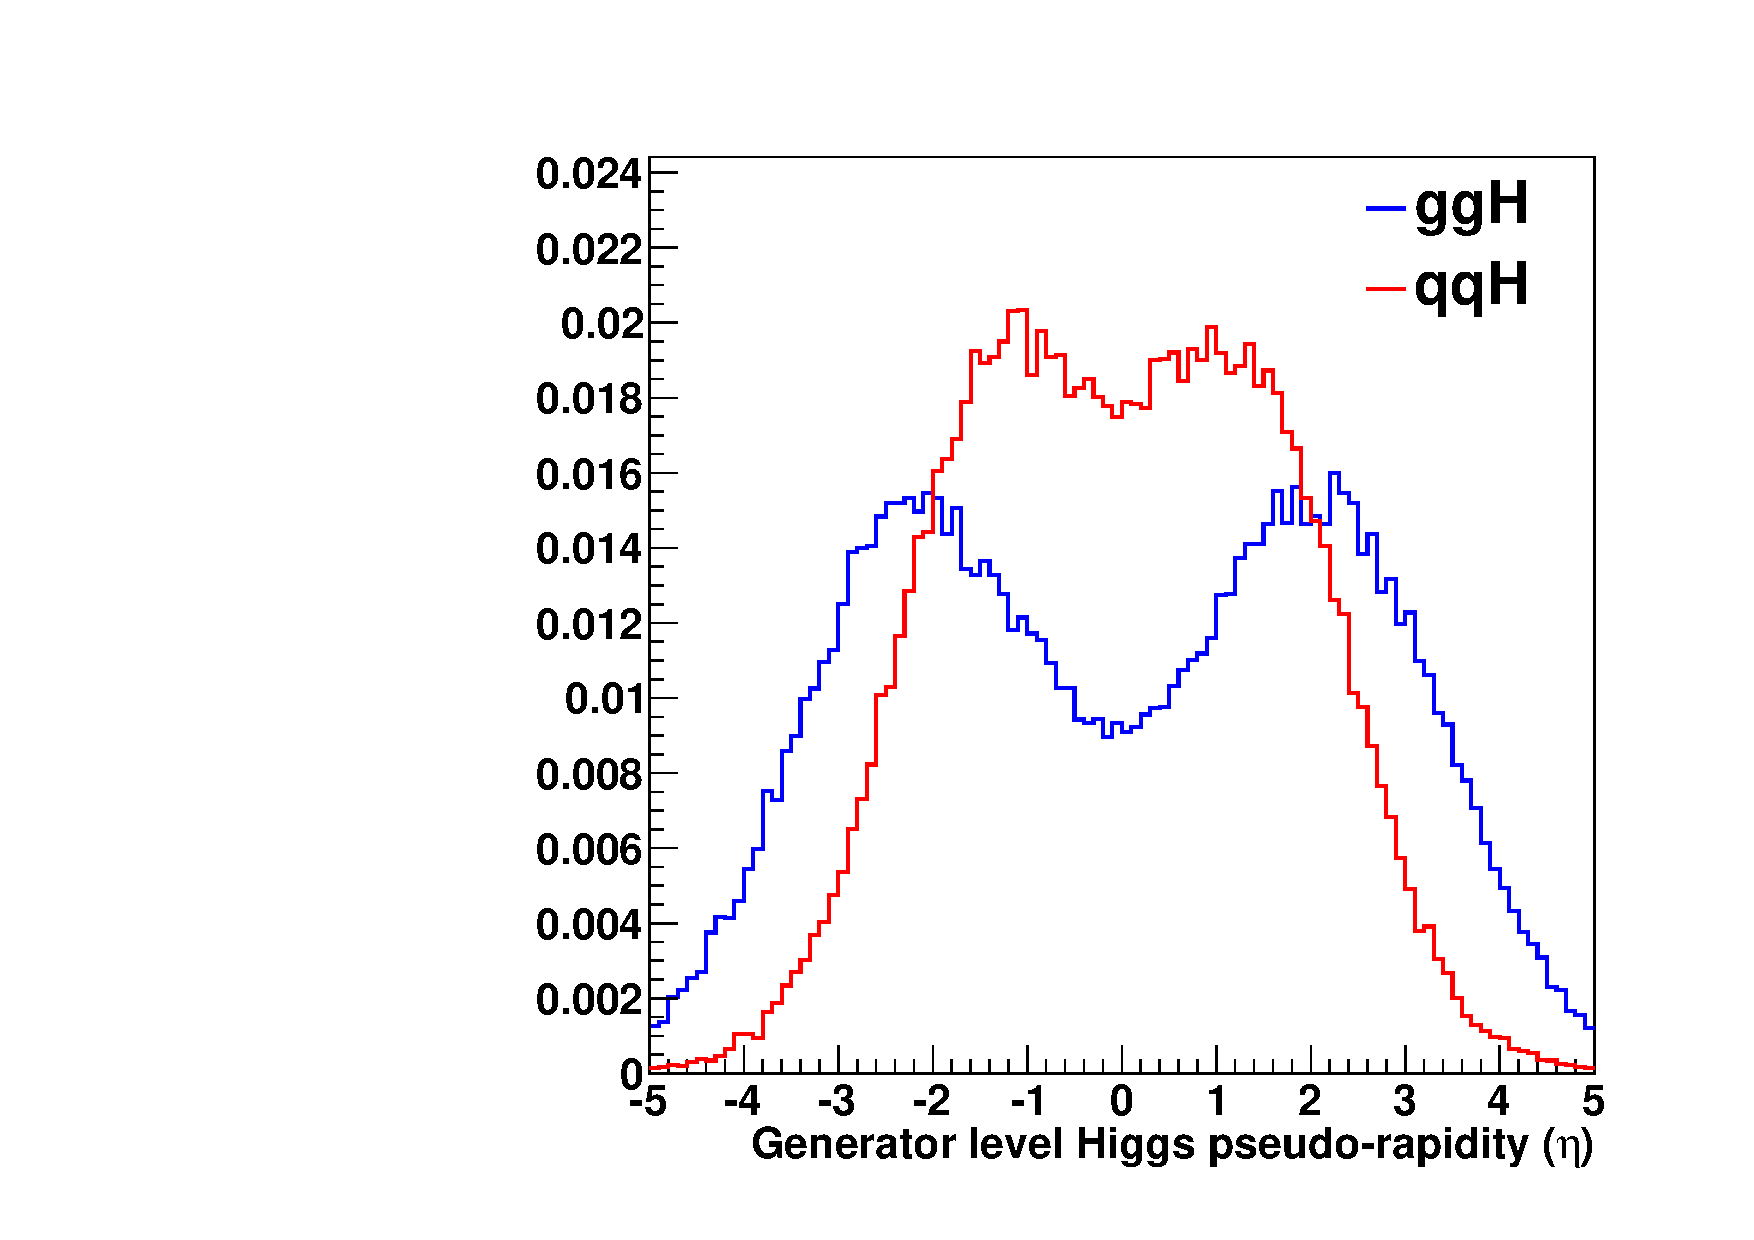
\includegraphics[width=0.45\textwidth]{theory/plots/genEta.pdf}
  \caption[Generator level Higgs distributions]{Generator level Higgs distribution in transverse momentum (left) and pseudorapidity (right) for production via gluon fusion (blue) and vector boson fusion (red) normalised to the same area.}
  \label{fig:gen_level}
\end{figure}

The \SM Higgs production cross section as a function of the Higgs mass, \mH, is shown for the low mass region $90\leq\mH\leq 300$~\GeV in Fig.~\ref{fig:higgs_xs} for centre-of-mass energies, $\sqrt{s}=7$ and 8~\TeV as provided by the LHC Higgs Cross Section Working Group~\cite{LHCHiggsCrossSectionWorkingGroup3}. It is clear that the production is dominated by \ggH but also that this mechanism has a large theoretical uncertainty. Once the statistics of the \LHC data become very high, this theoretical uncertainty becomes one of the dominant uncertainties in a cross section measurement. For a \SM Higgs boson with mass \mH=125~\GeV the cross section is about 18 (22)~pb for $pp$ collisions at $\sqrt{s}=$7 (8)~\TeV.

\begin{figure}
  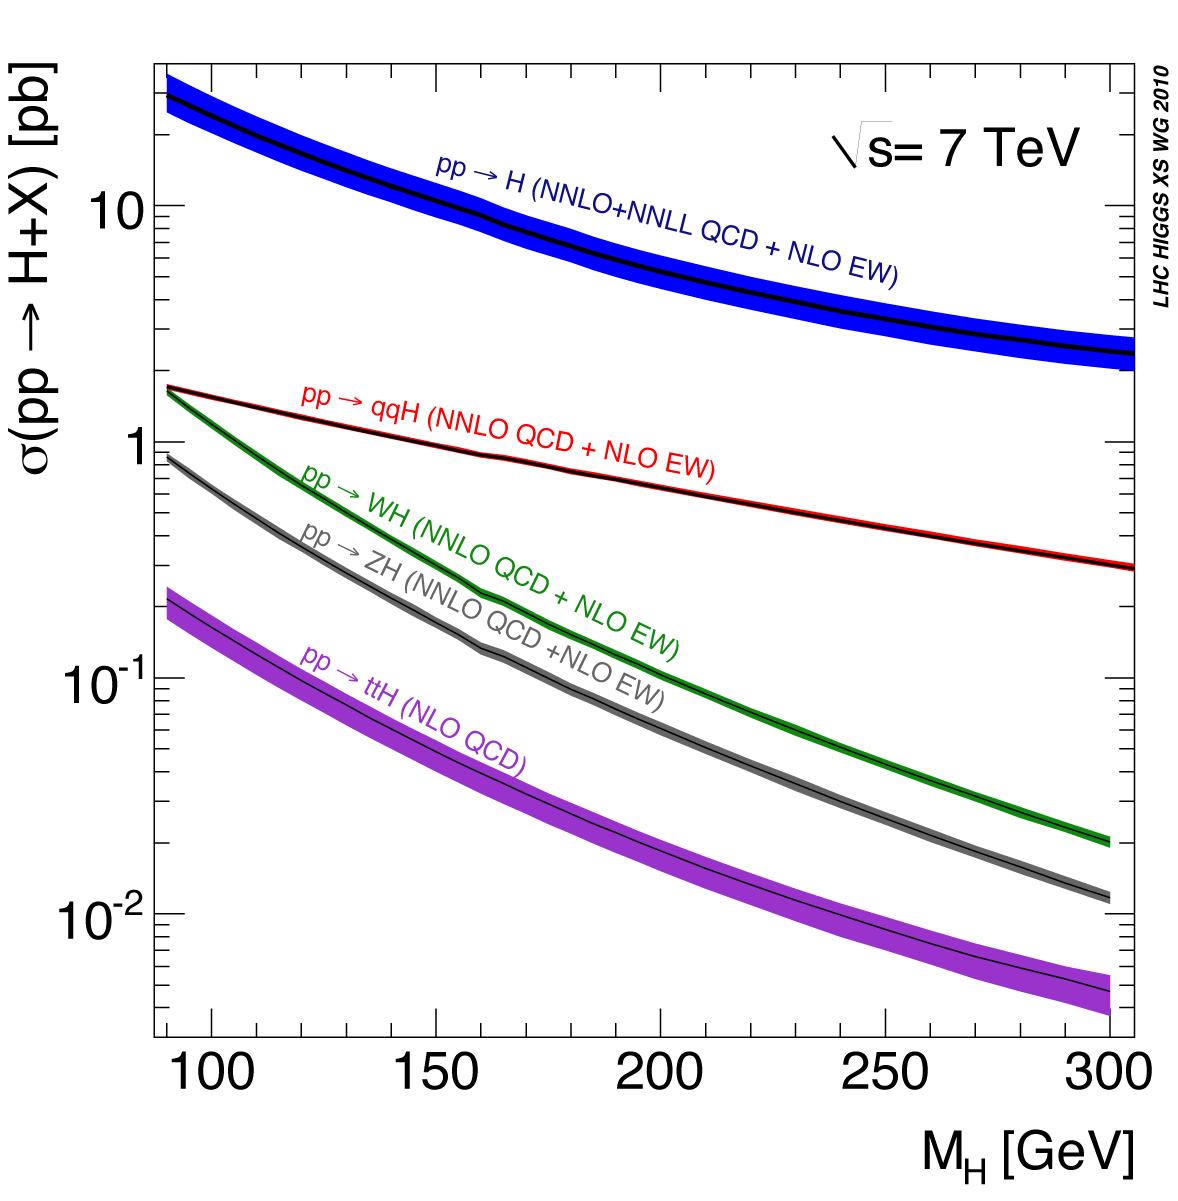
\includegraphics[width=0.48\textwidth]{theory/plots/Higgs_XS_7TeV_LM}
  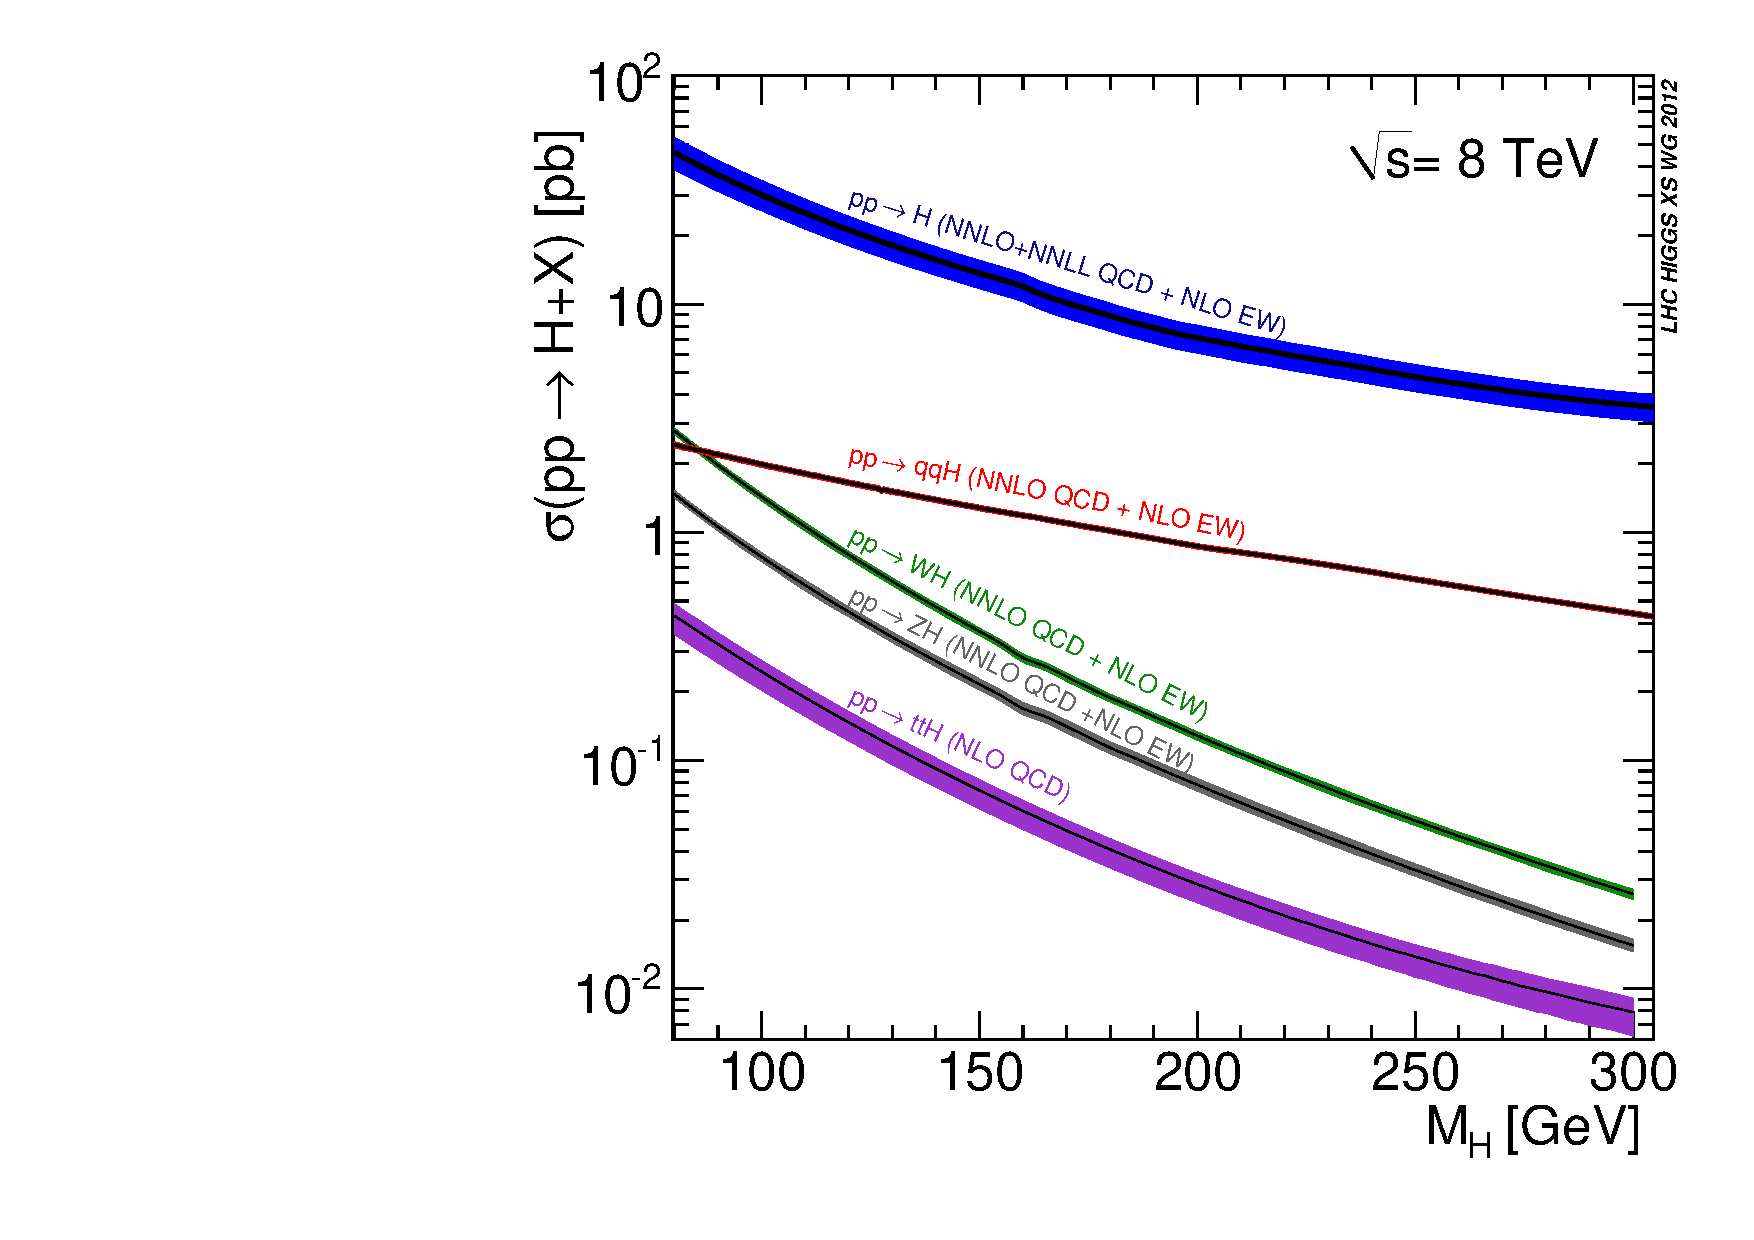
\includegraphics[width=0.48\textwidth]{theory/plots/Higgs_XS_8TeV_LM}
  \caption[\acs{SM} Higgs production cross section at the \acs{LHC}]{The \SM Higgs production cross section in proton-proton collisions at the \LHC for centre-of-mass energies of $\sqrt{s}=7$~\TeV (left) and $\sqrt{s}=8$~\TeV (right). The theoretical uncertainties on the values are shown as the coloured bands. Lines are shown for \ttH production (purple), \ZH production (grey), \WH production (green), \VBF production (red) and \ggH production (blue)~\cite{LHCHiggsCrossSectionWorkingGroup3}.}
  \label{fig:higgs_xs}
\end{figure}

\section{Higgs decay into two photons}

The Higgs couplings are proportional to the mass of the coupling object. Given the photon is massless there is no direct coupling between it and the Higgs. Consequently Higgs decays to photons occur via loop diagrams with $W$ bosons or quarks. For the latter, only the top quark loop need be considered given that the coupling is proportional to the mass and the top quark is considerably heavier than any of the other quarks. The Feynman diagrams for these processes at leading order are shown in Fig.~\ref{fig:feyn_hgg_decay}.

\begin{figure}
  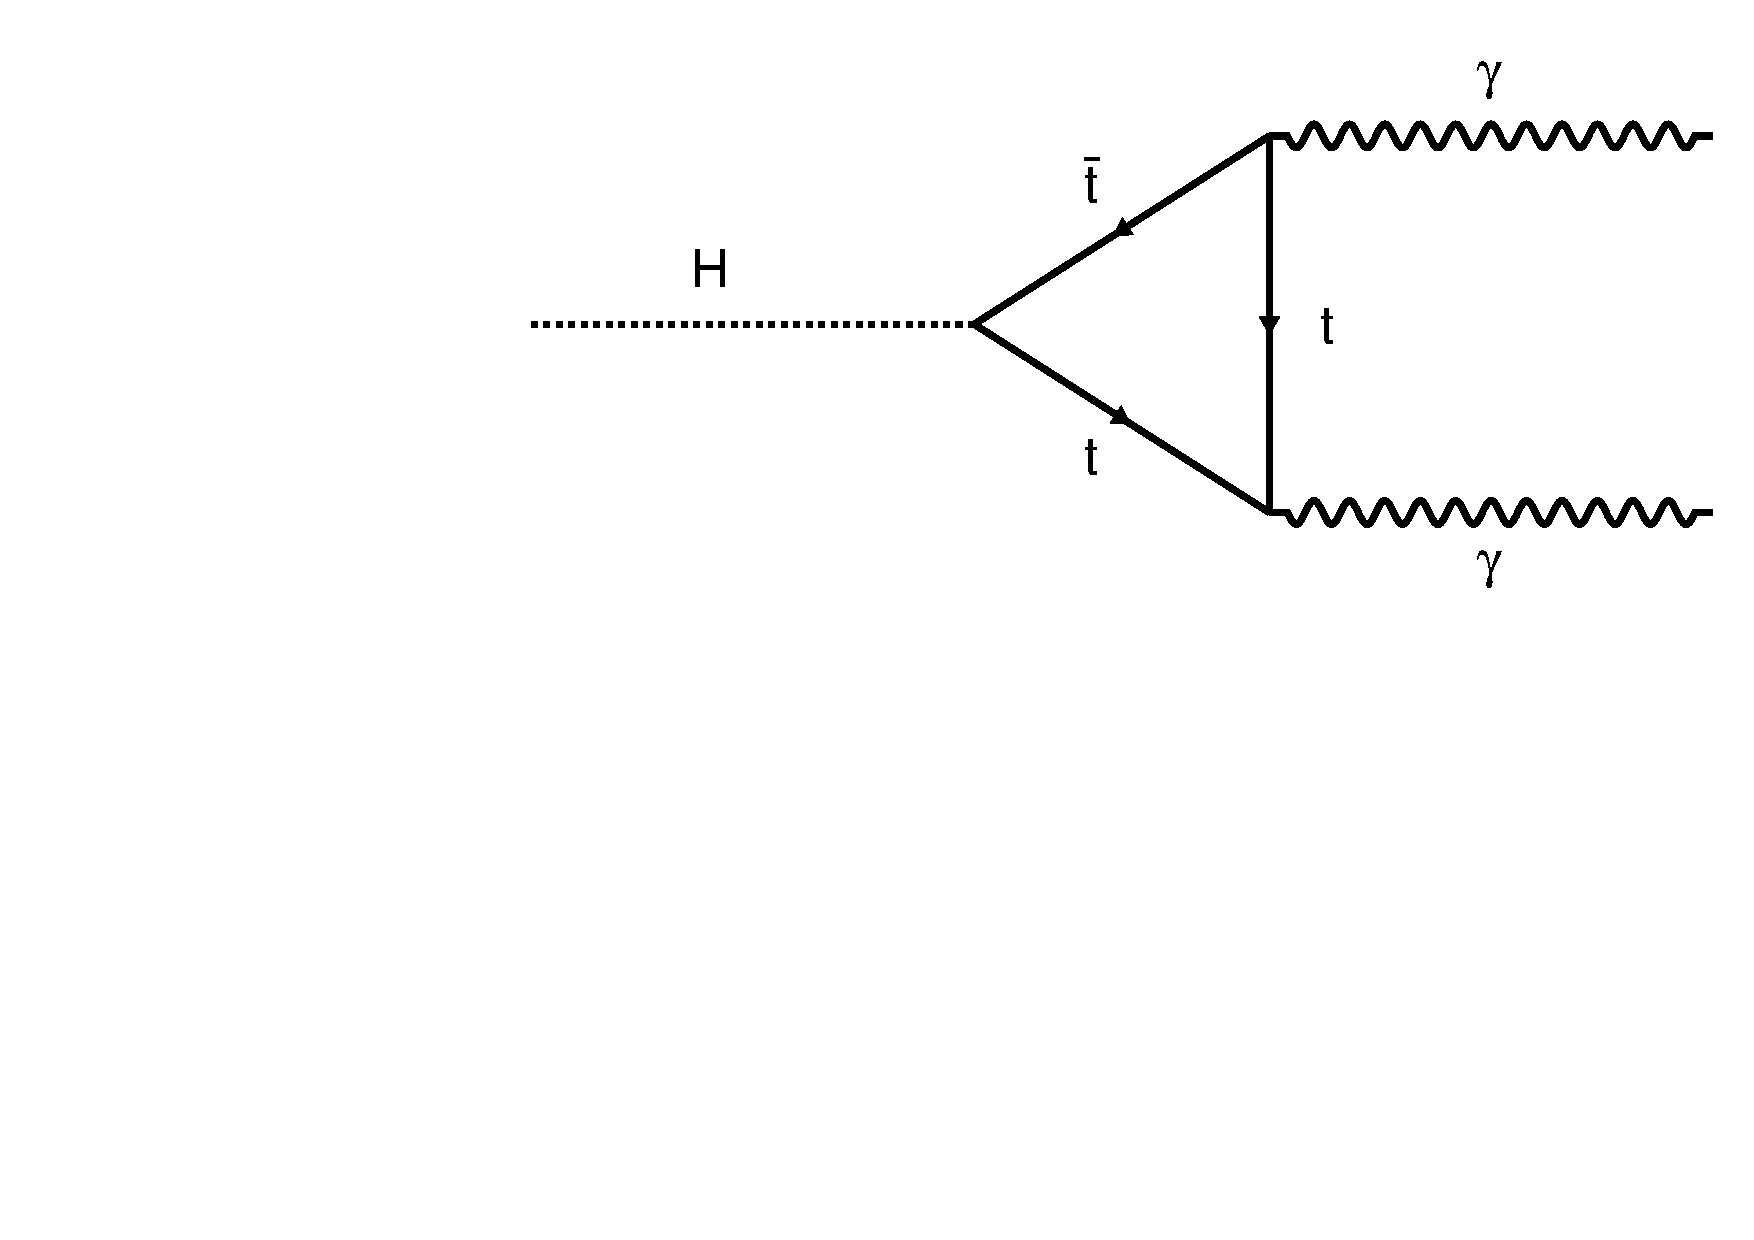
\includegraphics[width=0.32\textwidth]{theory/plots/Htgg.pdf}
  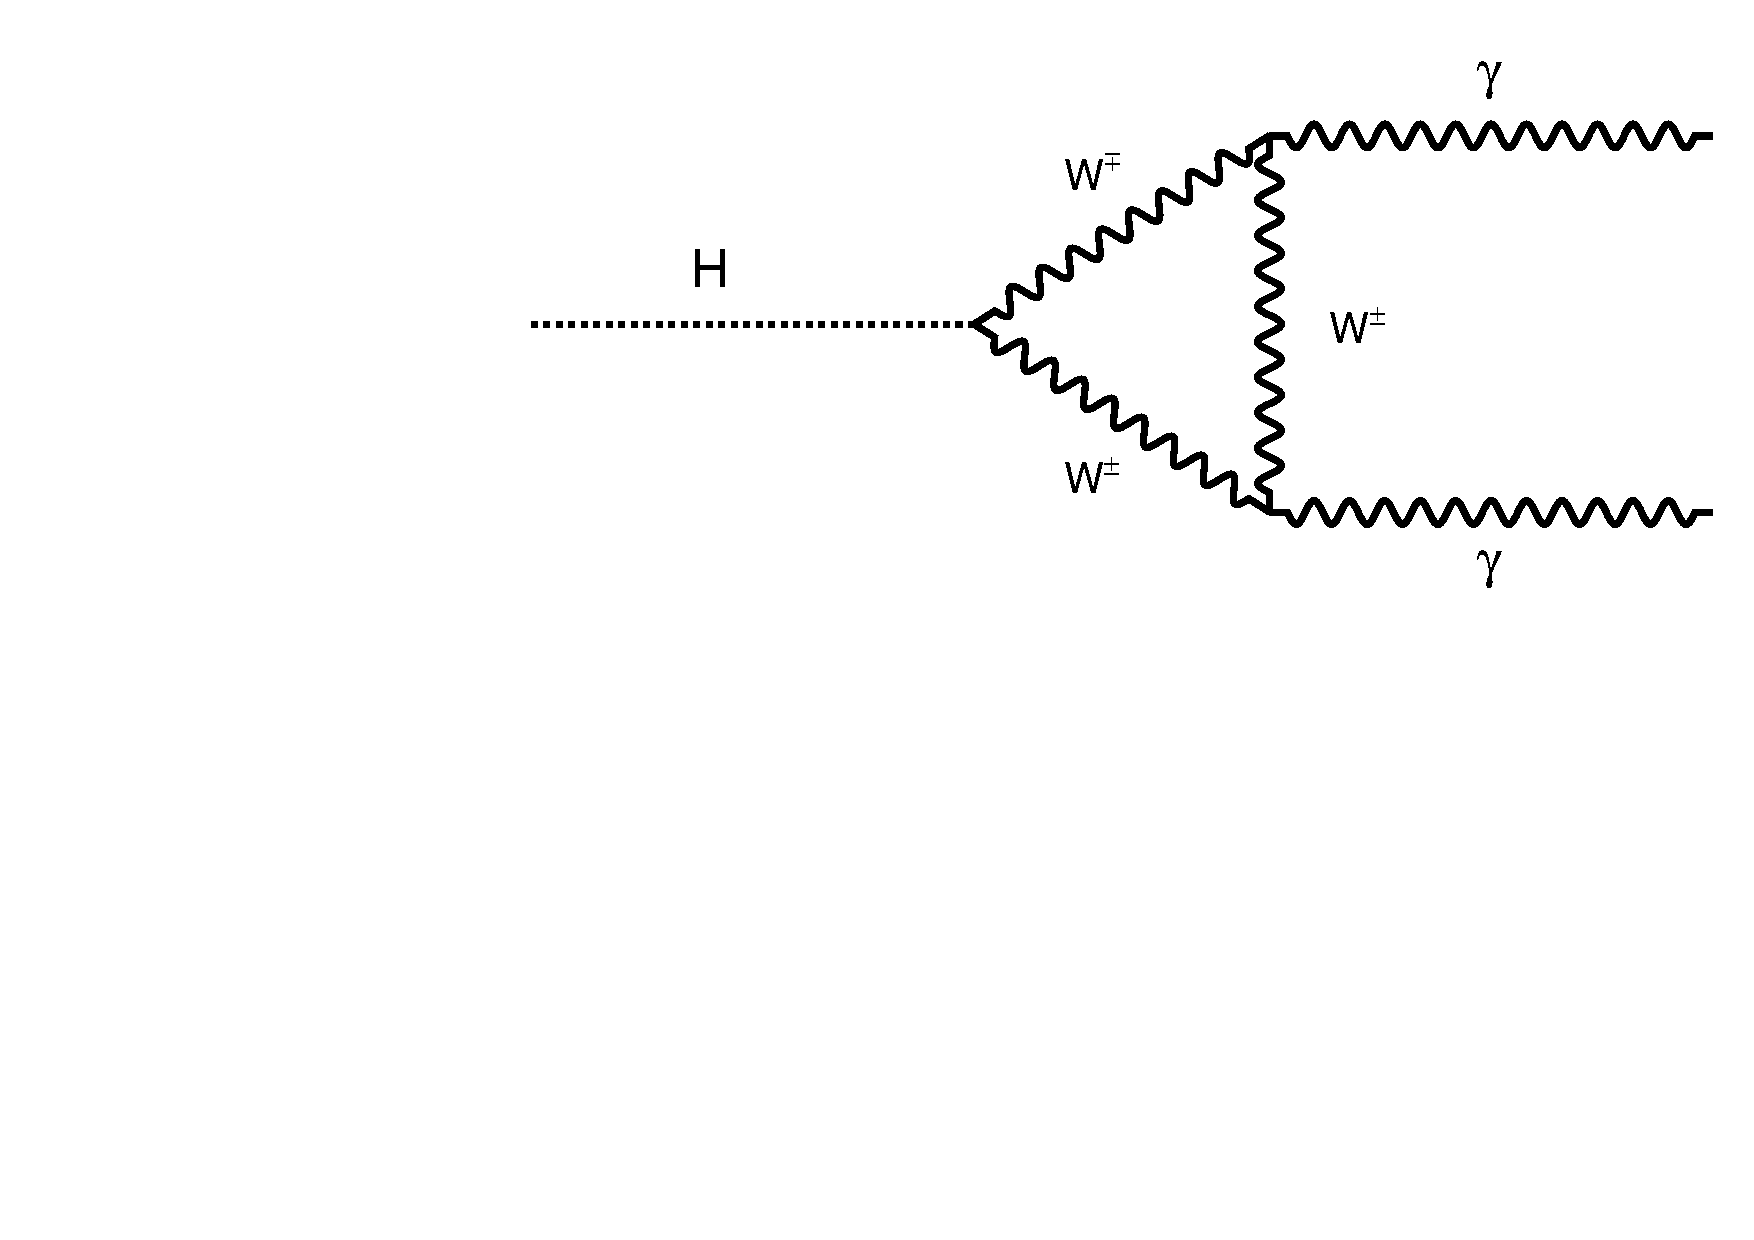
\includegraphics[width=0.32\textwidth]{theory/plots/HWgg.pdf}
  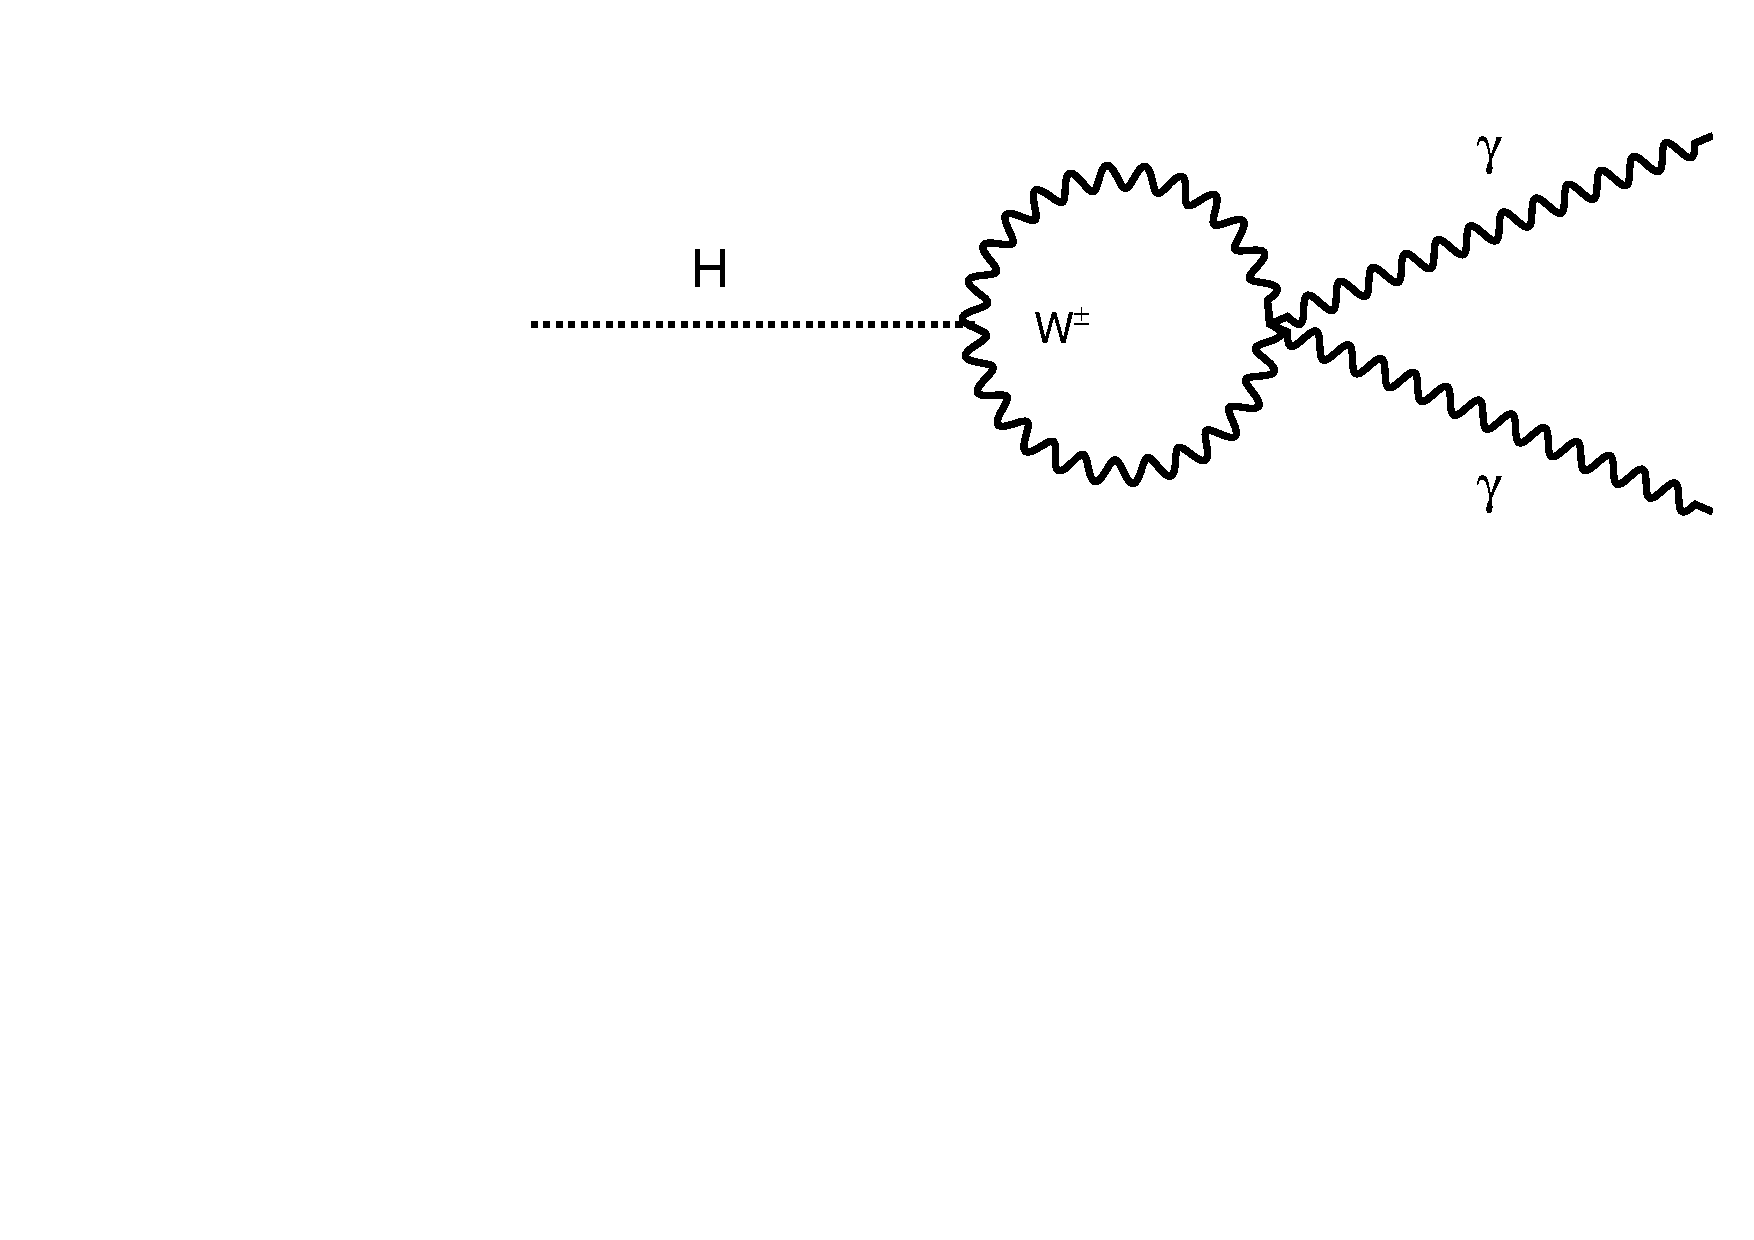
\includegraphics[width=0.32\textwidth]{theory/plots/HWgg4.pdf}
  \caption{Feynman diagrams for the \acs{SM} Higgs to two photon decay at leading order.}
  \label{fig:feyn_hgg_decay}
\end{figure}


The \SM Higgs branching ratio for each set of decay products is shown as a function of the Higgs mass, \mH, for the low mass region $80\leq\mH\leq 200$~\GeV in Fig.~\ref{fig:higgs_br} as provided by the LHC Higgs Cross Section Working Group~\cite{LHCHiggsCrossSectionWorkingGroup3}. The work in this thesis focuses on the Higgs decay into two photons (\Hgg) whose branching fraction is shown by the pink line. It is apparent that \Hgg decays are rare. There is only a small window of Higgs masses in which \Hgg decay is even feasible (\mH$<\sim185$~\GeV) and the peak of the branching fraction ($120<\mH<130$~\GeV) only allows a \SM \Hgg decay 0.2\% of the time. Given that the \LHC Run 1 dataset used in this thesis consists of 5.1\fbinv at \sqrts=7~\TeV and 19.7\fbinv at \sqrts=8~\TeV one can expect about 1/2 million \SM Higgs boson to be produced (assuming a value of \mH=125~\GeV) of which only about 1000 decay into two photons. 

\begin{figure}
  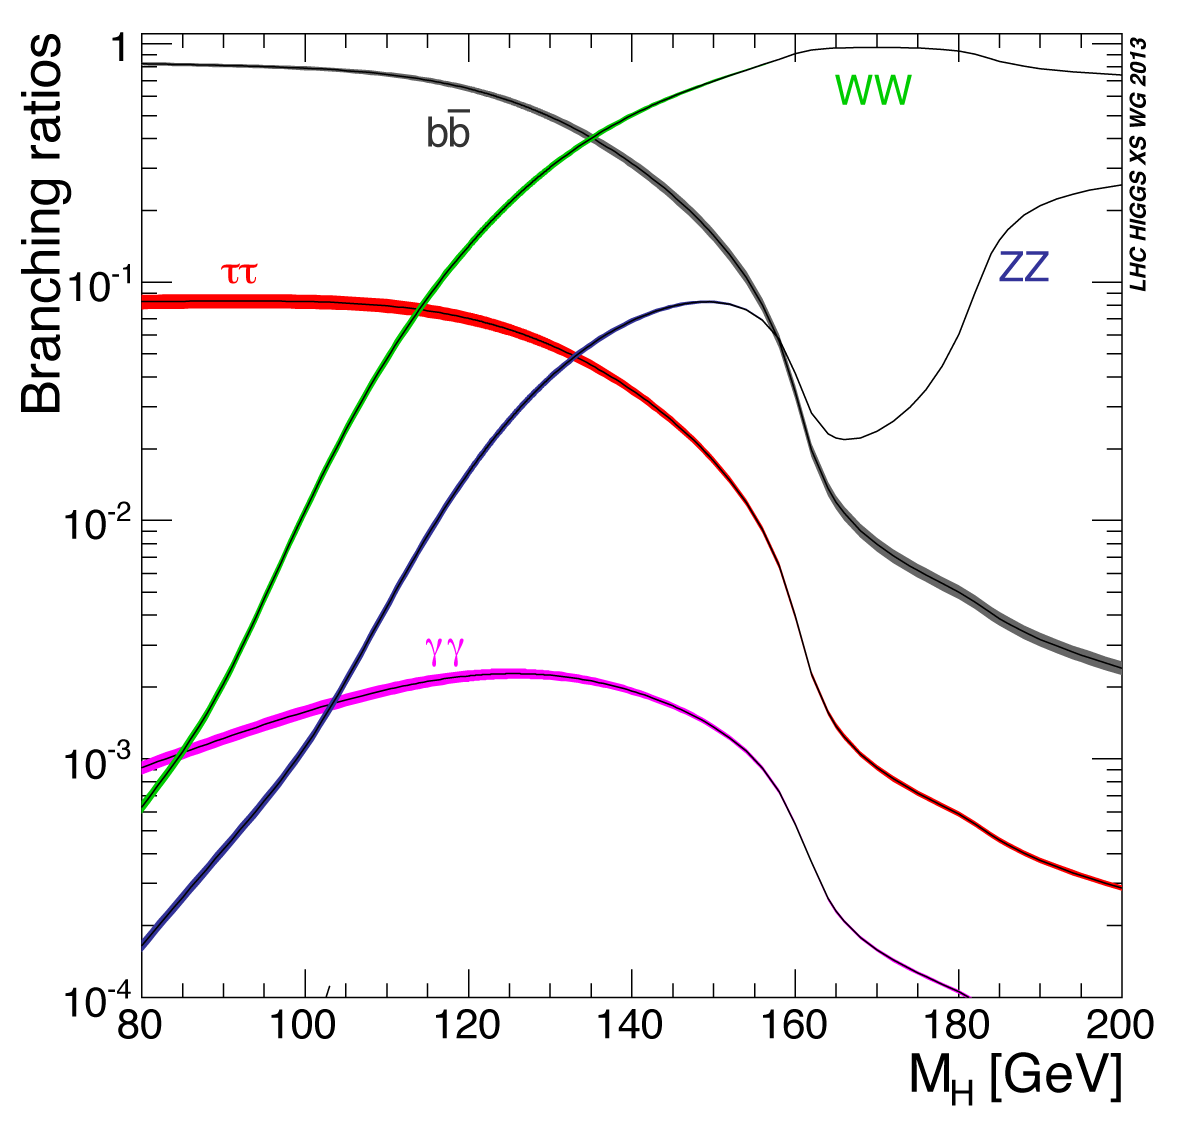
\includegraphics[width=0.6\textwidth]{theory/plots/Higgs_BR_LM}
  \caption[\acs{SM} Higgs branching fraction]{A plot showing the branching ratio of the \SM Higgs boson into various decay products as a function of the Higgs mass \mH. The theoretical uncertainties are shown as the coloured bands. Only the primary search channels are left on this figure (Higgs decaying into $b\bar{b}$, $ZZ$, $WW$, $\tau\tau$ and $\gamma\gamma$) for ease of viewing. There are several other possibilities left out (Higgs decaying into $gg$, $c\bar{c}$, $Z\gamma$, $\mu\mu$). This thesis concentrates on the \Hgg decay shown as the pink line~\cite{LHCHiggsCrossSectionWorkingGroup3}.}
  \label{fig:higgs_br}
\end{figure}

\subsection{Backgrounds to the \Hgg decay at the \LHC}

Aside from the very low signal rate of Higgs decays to two photons, further complications arise by considering the incredibly high rate of the background processes for two photon production in proton-proton collisions. A pair of real (prompt) photons is predominantly produced by \QCD interactions from a proton-proton initial state via two diagrams; the so-called Born ($q\bar{q}\rightarrow\gamma\gamma$) and the box ($gg\rightarrow\gamma\gamma$), collectively known as \textit{prompt-prompt} background. These two backgrounds are referred to as irreducible as they fake signal with two real photons. By using the specific kinematics of Higgs decays these backgrounds can be somewhat suppressed but the main challenge of the analysis is estimating the contamination of these processes in the signal region. The other type of background arises from final state neutral hadrons faking photons. Predominantly these are $\pi^{0}$s decaying into two almost collinear photons which fake the single photon signal. This can happen in association with one real photon, \gjet (known as \textit{prompt-fake}), or where both photons are faked by jet signals (known as \textit{fake-fake}). Nearly all of the \textit{fake-fake} background can be removed using the analysis techniques described in Chapters~\ref{chap:common_analysis_components} and~\ref{chap:selection_and_categorisation} such that the final analysis consists of about 70\% prompt-prompt, 30\% prompt-fake and $<1\%$ fake-fake. The Feynman diagrams for Born, box and \gjet production are shown in Fig.~\ref{fig:feyn_bkgs}.

\begin{figure}
  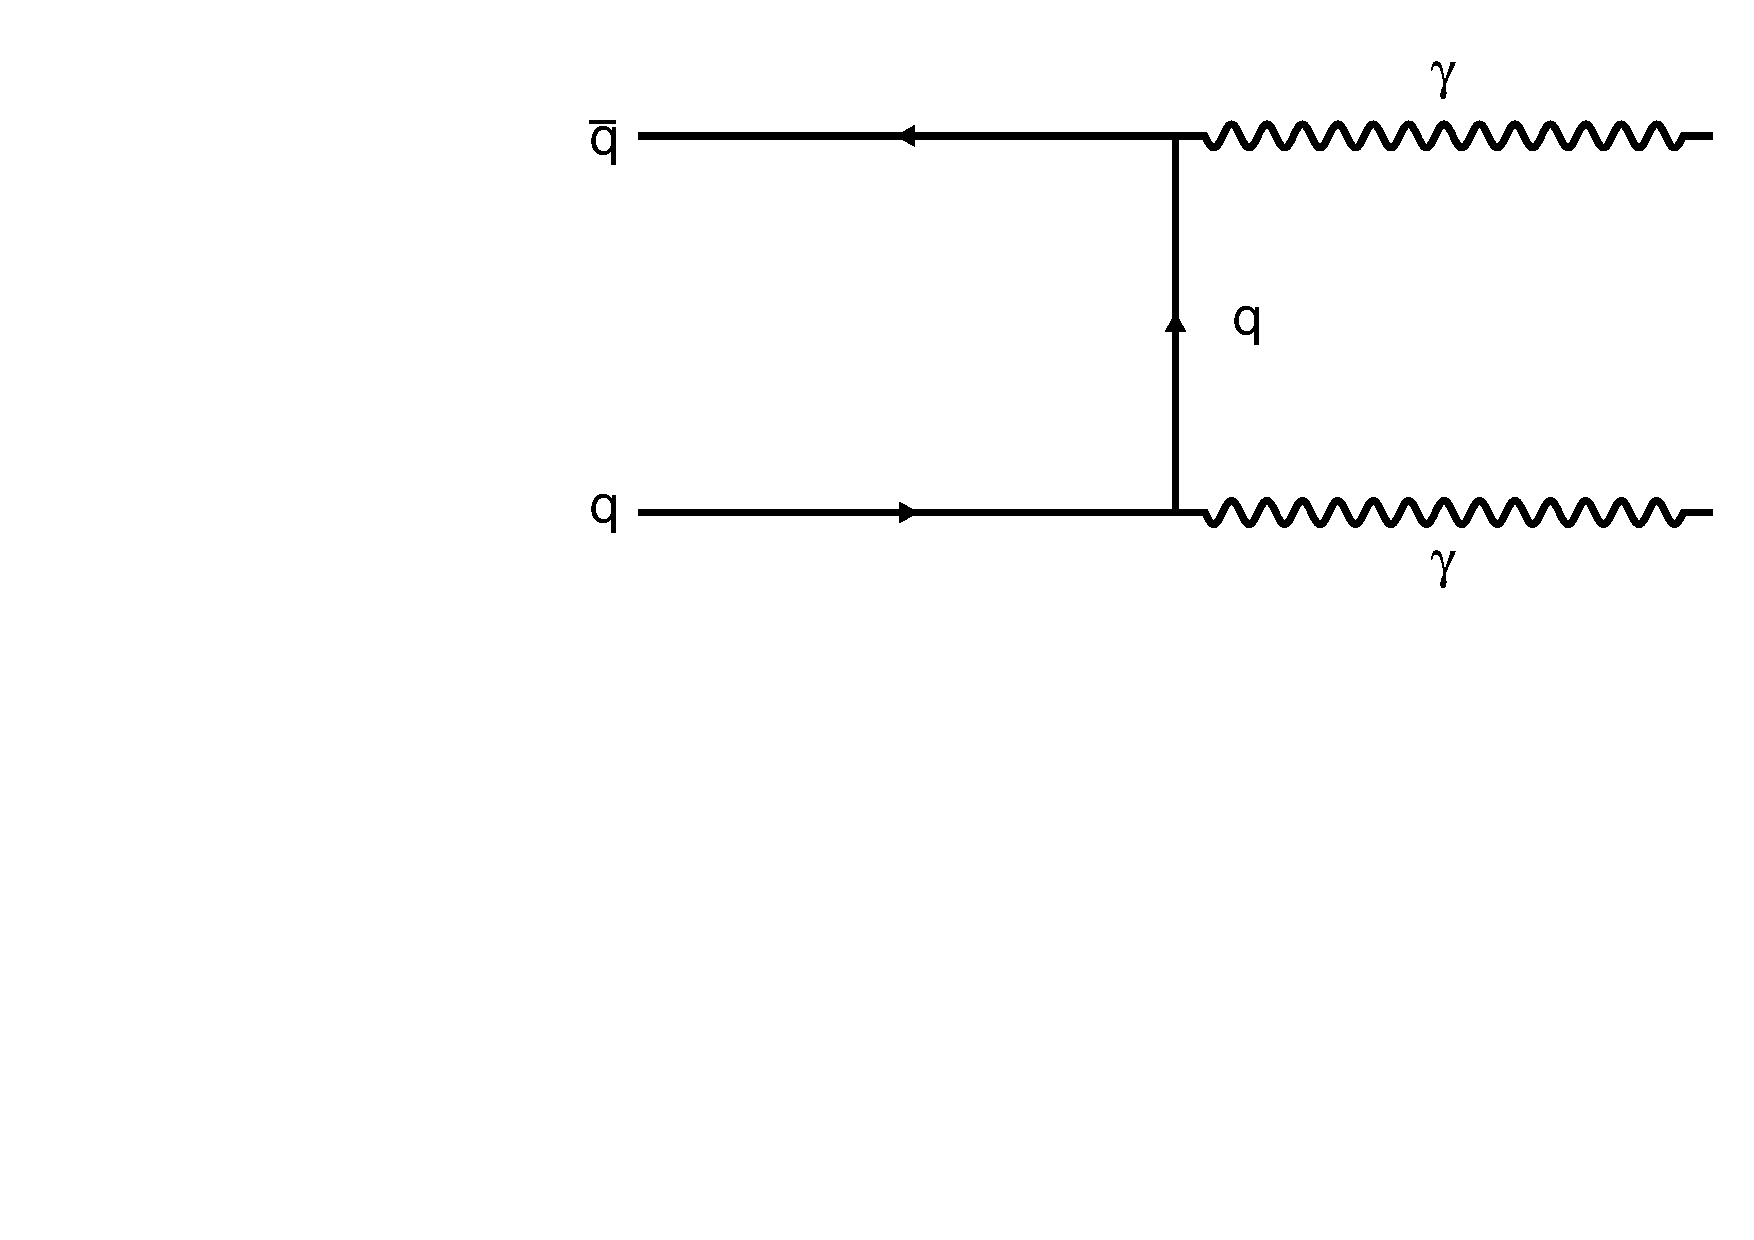
\includegraphics[width=0.32\textwidth]{theory/plots/Born.pdf}
  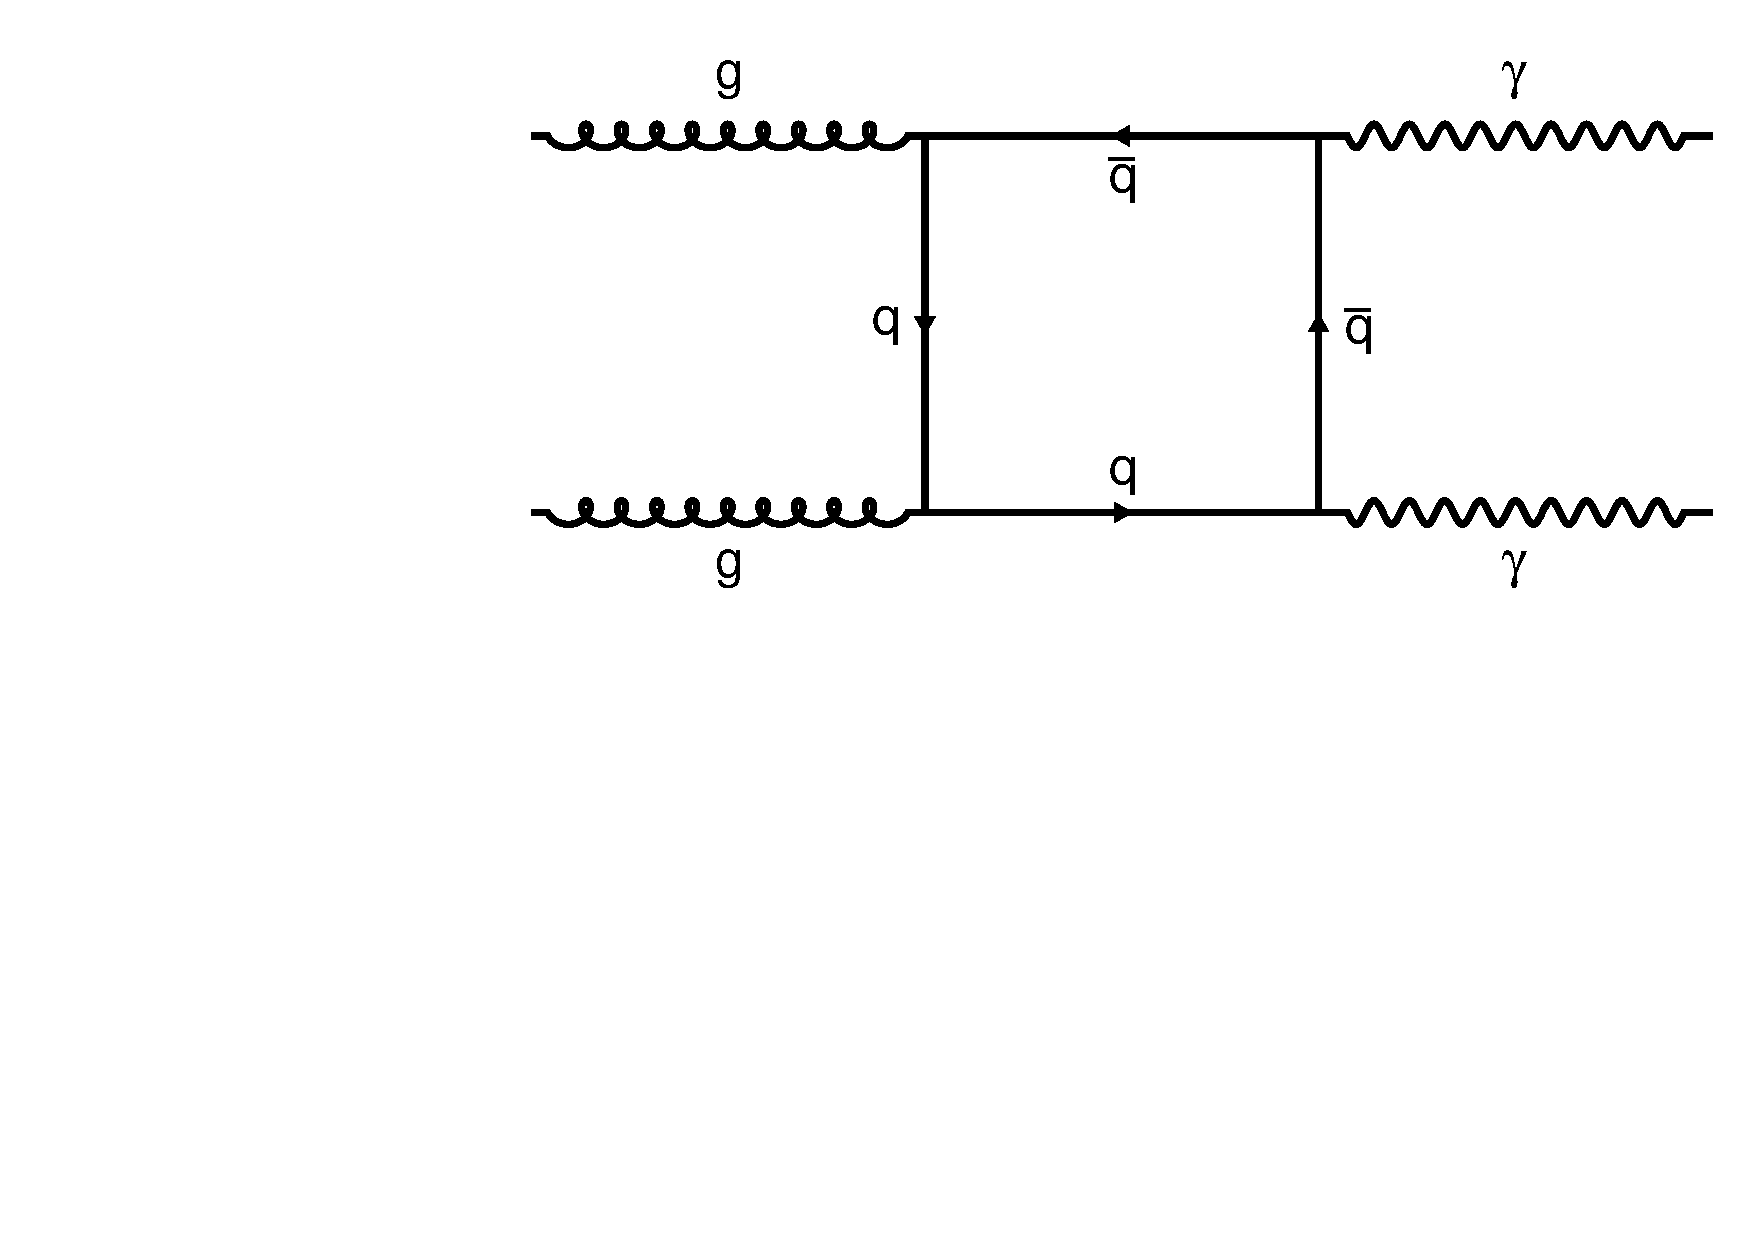
\includegraphics[width=0.32\textwidth]{theory/plots/Box.pdf}
  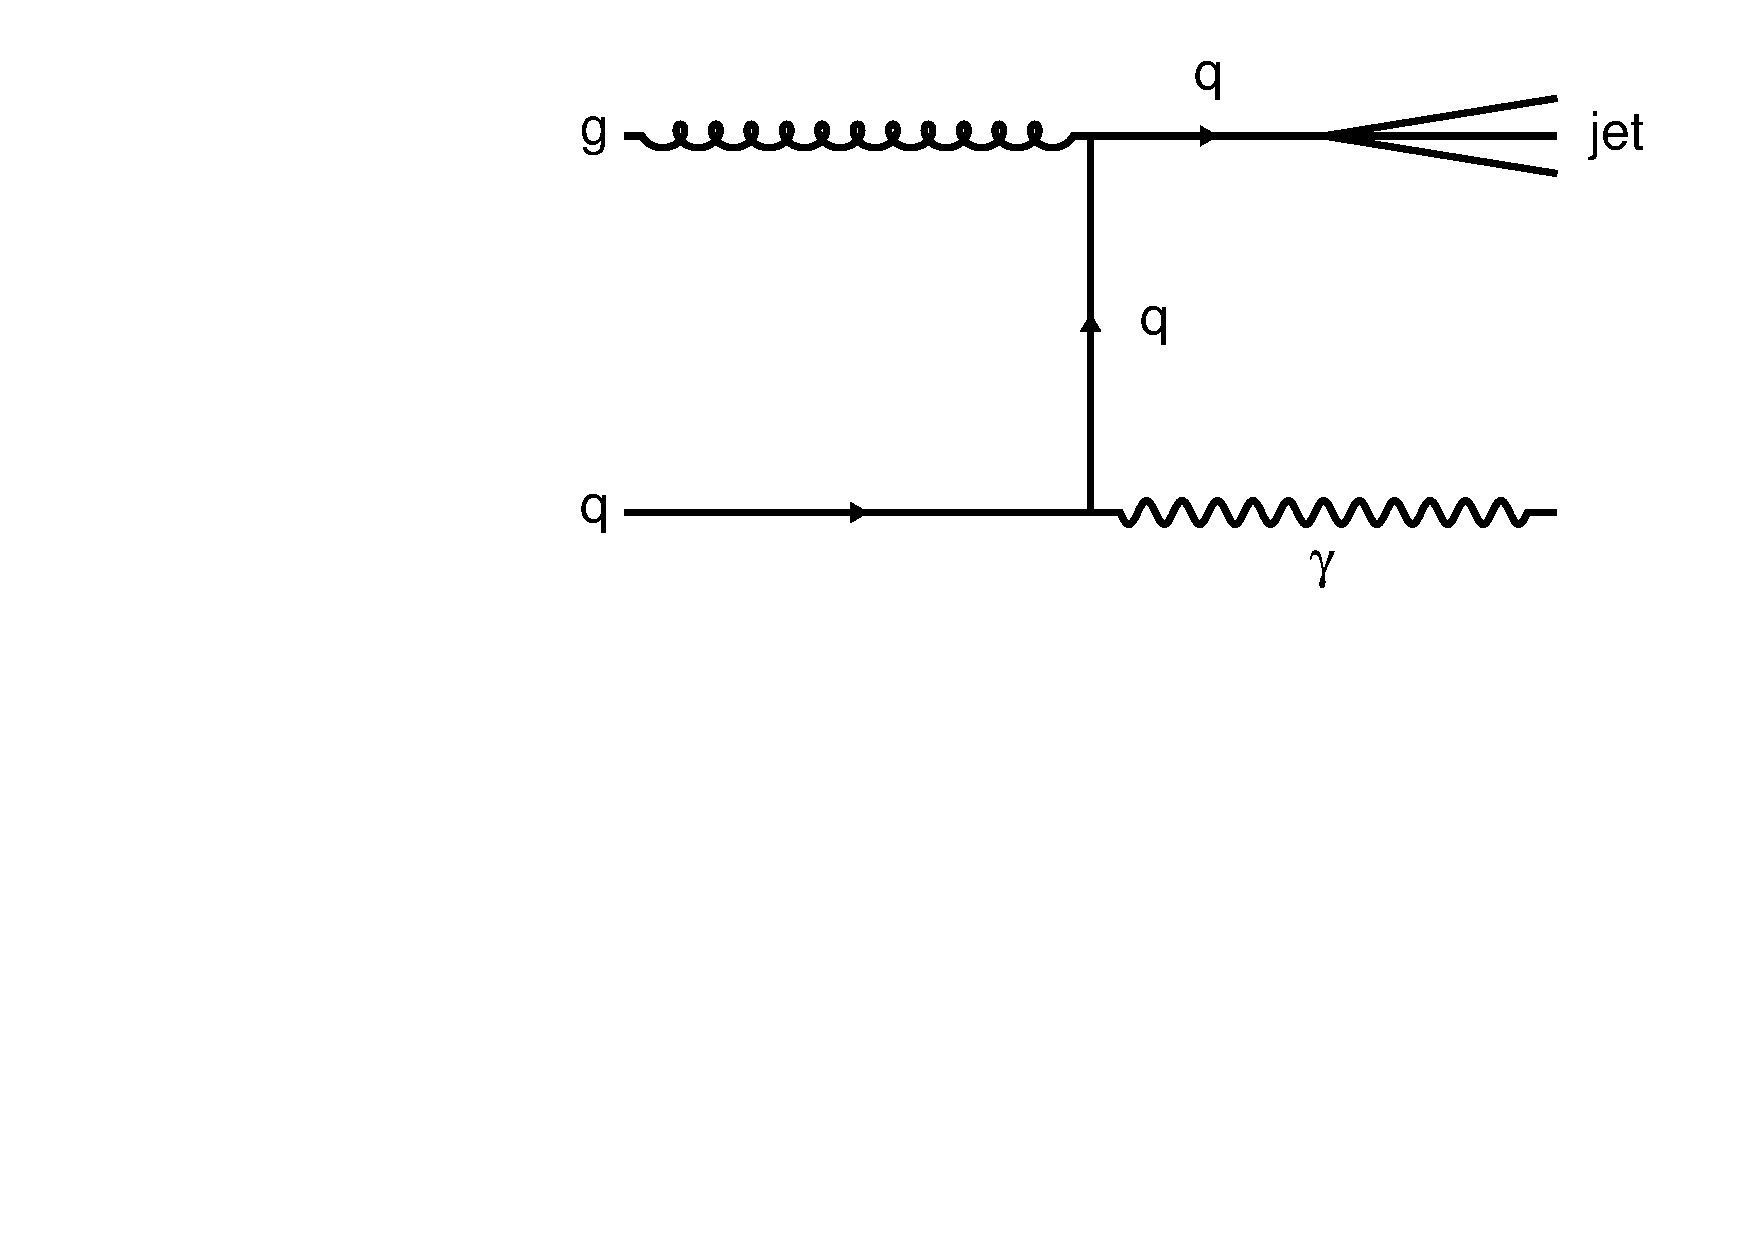
\includegraphics[width=0.32\textwidth]{theory/plots/GJet.pdf}
  \caption[Higgs to two photon backgrounds at the \acs{LHC}]{The prompt-promt and prompt-fake Feynman diagrams contributing to the \Hgg background via the Born mode (left), box mode (middle) and \gjet mode (right).}
  \label{fig:feyn_bkgs}
\end{figure}

One of the most important variables used in the analysis is the invariant mass of the two photons, which for signal is equivalent to the reconstructed Higgs mass. The invariant mass distribution for background is expected to be a smoothly falling continuum whereas the signal is expected to be a narrow resonance centred at the Higgs mass. The difference between these is heavily exploited in the analysis. The diphoton invariant mass is reconstructed using,
\begin{equation}
	m_{\gamma\gamma} = \sqrt{2E_{1}E_{2}(1-\cos\alpha)},
\label{eq:invmass}
\end{equation}
where $E_{1}$ and $E_{2}$ are the energies of the two photons, and $\alpha$ is the angle between them.

The remainder of this thesis will concentrate on the details of an analysis of Higgs events decaying into two photons at the \CMS experiement at the \LHC. Many of the features discussed in the last section will be exploited using sophisticated computing, analysis and statistical techniques which ultimately culminate in a standalone observation of a resonance near 125~\GeV and subsequent measurements of this particle's properties.

